\chapter{Resultados}

\section{Alinhamento e Análise de Exomas}

No dia 6 de outubro de 2011 foi recebido o primeiro exoma para ser analisado pelo Laboratório de Genômica Clínica (LGC) na Faculdade de Medicina da UFMG em Belo Horizonte.

O sequenciamento desse exoma foi realizado utilizando um sequenciador modelo Illumina HiSeq2000, utilizando o kit de enriquecimento para captura das regiões exônicas desenvolvido pela Roche NimbleGen versão SeqCap EZ Human Exome Library v2 (44.1 Mbp) e foi dada uma garantia de cobertura mínima de pelo menos 30 vezes (30X) pela empresa Otogenetics que realizou o sequenciamento do DNA deste paciente.

Após o recebimento dos dois arquivos em formato FASTQ.GZ nós utilizamos o programa FASTQC para verificar a quantidade de leituras e obter métricas em relação aos valores de qualidade das leituras deste indivíduo.

\subsection{Controle de Qualidade sobre os dados}

Esses dois arquivos FASTQ continham 35.701.713 \textit{leituras} cada um, totalizando 71.403.426 de ``\textit{leituras paired-end}'', essas leituras estavam codificadas com um escore phred de qualidade no formato Illumina 1.5+ e tiveram que ser convertidas para o formato Sanger de qualidade para se tornarem compatíveis com o programa GATK. Cada leitura possui 90 nucleotídeos de tamanho tanto para as sequências \textit{forward} quanto as \textit{reverse} e o conteúdo médio GC dessas sequências foi de 44\%. Este valor está próximo do valor de 50\% que seria o esperado para as regiões exônicas do genoma humano. Um valor muito alto ou muito baixo de GC poderia indicar que houve algum tipo de problema com o enriquecimento dessas regiões.

Na tabela \ref{rms_seq} são apresentadas informações sobre as sequências forward e reverse que foram obtidas utilizando o programa FASTQC. Esses arquivos é o que chamamos de dados brutos (``\textit{raw data}''), pois são os dados que saíram diretamente do sequenciador e ainda não foram analisados ou alterados por nenhum tipo de programa.

\afterpage{

\begin{landscape}

\begin{table}[!htb]
    \caption{Métricas sobre as Sequências \textit{forward} e \textit{reverse} do indivíduo RMS}
    \label{rms_seq}
    \begin{subtable}{.5\linewidth}
      \centering
        \caption{Forward}
        \scalebox{1.3}{
	  \begin{tabular}{|l|l|}
	  \hline
	  \multicolumn{1}{|c|}{\textbf{Medida}} & \multicolumn{1}{c|}{\textbf{Valor}} \\ \hline
	  Tipo de Arquivo & Conventional base calls \\ \hline
	  Codificação & Illumina 1.5 \\ \hline
	  Total de Sequências & 35.701.713 \\ \hline
	  Sequências Filtradas & 0 \\ \hline
	  Tamanho das Sequências & 90 \\ \hline
	  \%GC & 44 \\ \hline
	  \end{tabular}
	}
    \end{subtable}%
    \begin{subtable}{.5\linewidth}
      \centering
        \caption{Reverse}
        \scalebox{1.3}{
        \begin{tabular}{|l|l|}
	\hline
	\multicolumn{1}{|c|}{\textbf{Medida}} & \multicolumn{1}{c|}{\textbf{Valor}} \\ \hline
	Tipo de Arquivo & Conventional base calls \\ \hline
	Codificação & Illumina 1.5 \\ \hline
	Total de Sequências & 35.701.713 \\ \hline
	Sequências Filtradas & 0 \\ \hline
	Tamanho das Sequências & 90 \\ \hline
	\%GC & 44 \\ \hline
	\end{tabular}
	}
    \end{subtable} 
\end{table}

\end{landscape}


\clearpage
}

A seguir são apresentadas imagens com informações sobre a qualidade das leituras. Podemos observar que esses dados estão com um valor ótimo de qualidade e não possuem nenhum desvio significativo em relação aos valores que seriam esperados.

Na figura \ref{fig:per_base_sequence_quality} podemos observar que a qualidade das bases ao longo das leituras possui em média um \textit{phred escore} acima de 30 e notamos que a partir do meio da leitura até o seu final existe uma leve redução dos valores de qualidade, isto geralmente acontece com dados de sequenciadores Illumina.

A figura \ref{fig:per_sequence_quality} mostra a qualidade média das leituras e podemos observar que os valores de qualidade estão entre 37 e 38 tanto para a sequência forward quanto para a sequência reverse. Este resultado pode ser considerado bom, caso contrário esta imagem poderia indicar algum tipo de problema ocorrido durante o sequenciamento.

Na figura \ref{fig:per_base_sequence_content} apresentamos a distribuição dos nucleotídeos A, C, T e G ao longo das leituras e podemos observar que a quantidade de nucleotídeos A e T foi maior do que a quantidade de nucleotídeos G e C. Isso é esperado e pode ser considerado normal desde que a diferença entre esses dois grupos não ultrapasse 20\%.


\afterpage{
\begin{landscape}

\begin{figure}
\centering
\Large\textbf{Escore \textit{Phred} de qualidade médio por base das sequências do indivíduo RMS}\par\medskip   
\begin{subfigure}{.75\textwidth}
  \centering
  \fbox{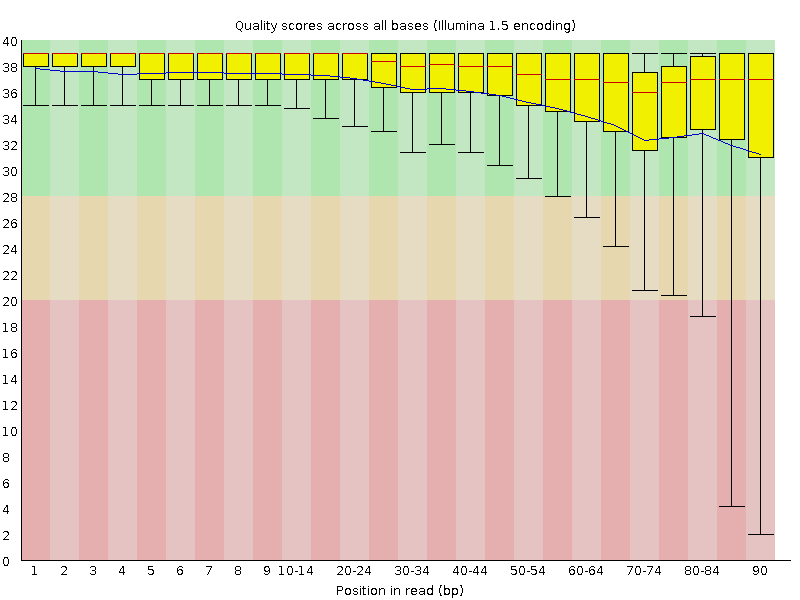
\includegraphics[width=0.9\linewidth]{../Figures/Ot729_index7_Exome_Sergio.Pena_RDNP_07262011-reads1-110716_I123_FCC043NABXX_L2_index7_1_fastqc/Images/per_base_quality.png}}
  \caption{Sequências Forward}
\end{subfigure}%
\begin{subfigure}{.75\textwidth}
  \centering
  \fbox{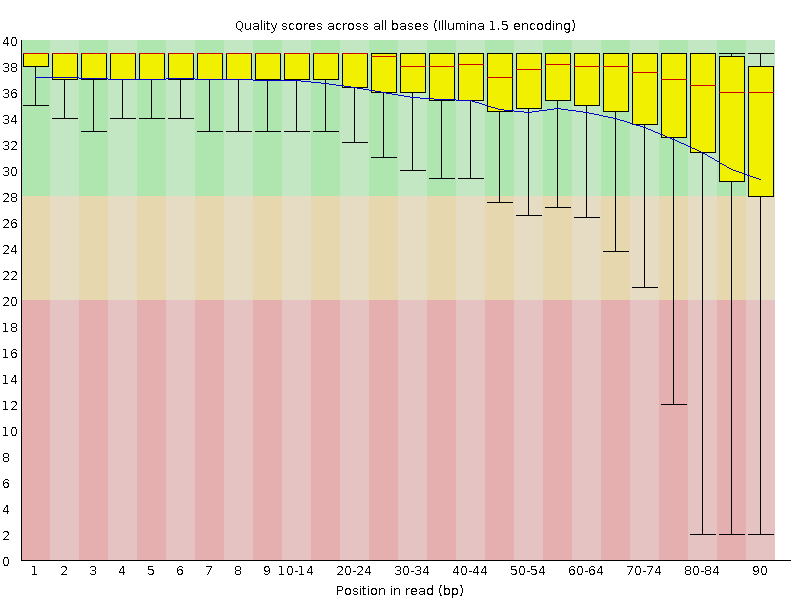
\includegraphics[width=0.9\linewidth]{../Figures/Ot729_index7_Exome_Sergio.Pena_RDNP_07262011-reads2-110716_I123_FCC043NABXX_L2_index7_2_fastqc/Images/per_base_quality.png}}
  \caption{Sequências Reverse}
\end{subfigure}
\caption[Escore \textit{Phred} de qualidade médio por base das sequências do indivíduo RMS]{Podemos observar que o score phred de qualidade das bases ficou sempre acima de 30, havendo uma pequena degradação no final das reads, o que é bastante característico de dados provenientes da plataforma illumina.}
\label{fig:per_base_sequence_quality}
\end{figure}

\begin{figure}
\centering
\Large\textbf{Distribuição do Escore \textit{Phred} em relação a todas as sequências do indivíduo RMS}\par\medskip   
\begin{subfigure}{.75\textwidth}
  \centering
  \fbox{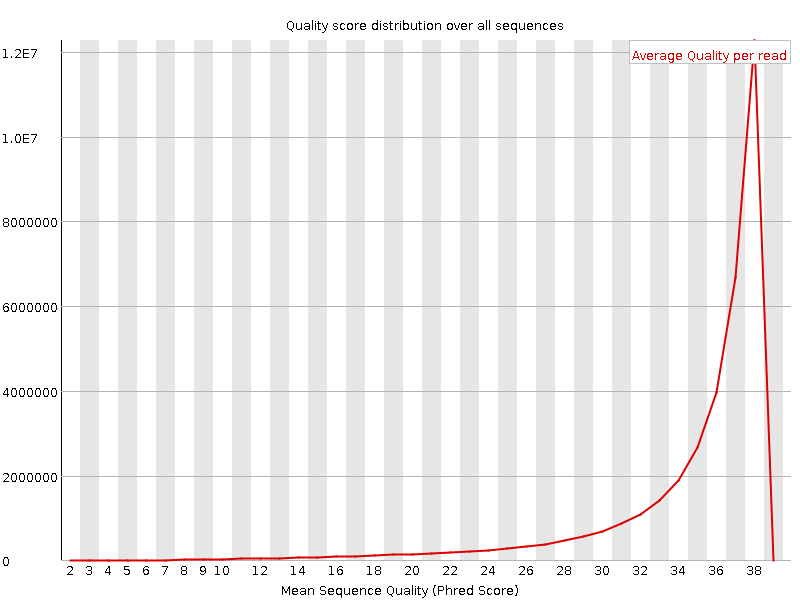
\includegraphics[width=0.9\linewidth]{../Figures/Ot729_index7_Exome_Sergio.Pena_RDNP_07262011-reads1-110716_I123_FCC043NABXX_L2_index7_1_fastqc/Images/per_sequence_quality.png}}
  \caption{Sequências Forward}

\end{subfigure}%
\begin{subfigure}{.75\textwidth}
  \centering
  \fbox{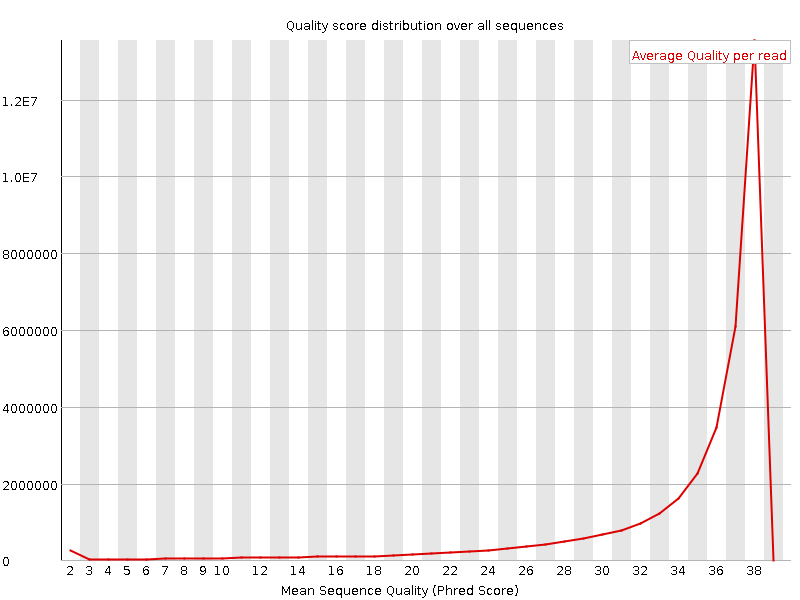
\includegraphics[width=0.9\linewidth]{../Figures/Ot729_index7_Exome_Sergio.Pena_RDNP_07262011-reads2-110716_I123_FCC043NABXX_L2_index7_2_fastqc/Images/per_sequence_quality.png}}
  \caption{Sequências Reverse}

\end{subfigure}
\caption[Distribuição do Escore \textit{Phred} em relação a todas as sequências do indivíduo RMS]{Podemos observar que o phred escore médio de qualidade para as reads forward e reverse foram de 38.}
\label{fig:per_sequence_quality}
\end{figure}

\begin{figure}
\centering
\Large\textbf{Conteúdo de sequência por base para as sequências do indivíduo RMS}\par\medskip
\begin{subfigure}{.75\textwidth}
  \centering
  \fbox{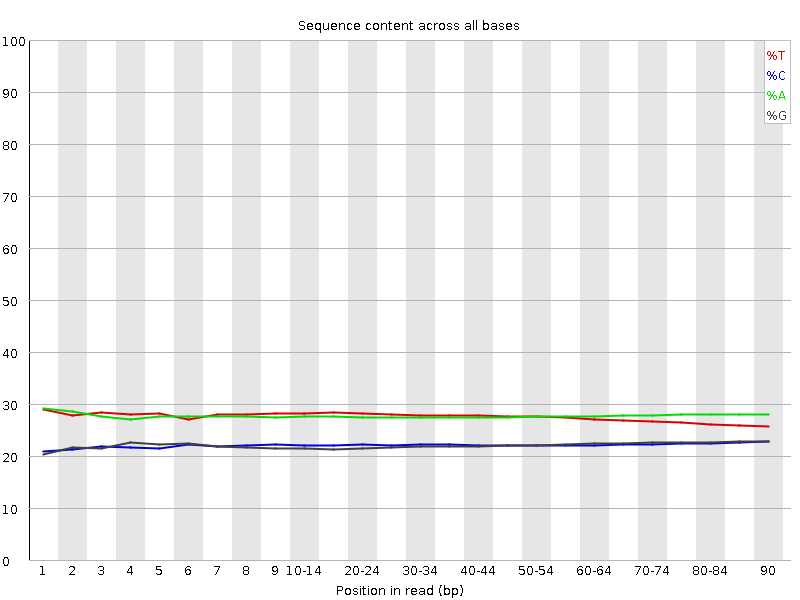
\includegraphics[width=0.9\linewidth]{../Figures/Ot729_index7_Exome_Sergio.Pena_RDNP_07262011-reads1-110716_I123_FCC043NABXX_L2_index7_1_fastqc/Images/per_base_sequence_content.png}}
  \caption{Sequências Forward}
\end{subfigure}%
\begin{subfigure}{.75\textwidth}
  \centering
  \fbox{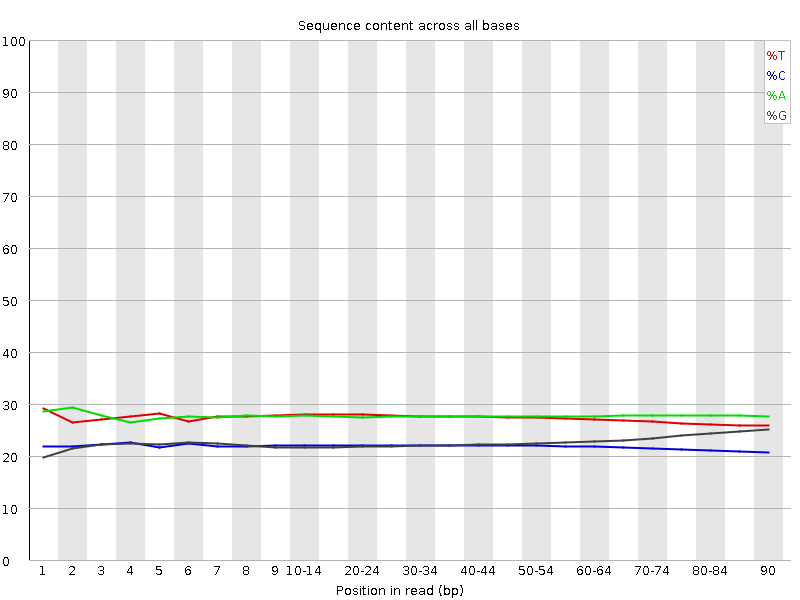
\includegraphics[width=0.9\linewidth]{../Figures/Ot729_index7_Exome_Sergio.Pena_RDNP_07262011-reads2-110716_I123_FCC043NABXX_L2_index7_2_fastqc/Images/per_base_sequence_content.png}}
  \caption{Sequências Reverse}
\end{subfigure}
\caption[Conteúdo de sequência por base para as sequências do indivíduo RMS]{Nesta figura podemos observar a distribuição de cada uma das bases A, C, T, e G ao longo das reads.}
\label{fig:per_base_sequence_content}
\end{figure}

\end{landscape}

}

Na figura \ref{fig:gc_content_per_sequence} podemos observar a distribuição do conteúdo GC para todas as sequências e que esse valor foi em média 44\%. A linha em azul representa o modelo teórico de distribuição que seria esperado. Podemos afirmar que o valor real aproxima-se bastante do valor esperado e caso estas distribuições fossem diferentes isso poderia indicar um problema de contaminação da amostra com outros organismos.

Na figura \ref{fig:duplication_levels} apresentamos os níveis de duplicação das sequência e podemos observar valores de duplicação de 39.79\% e 38.73\% para as sequências, o que pode ser considerado baixo. Um alto nível de duplicação indica que houve um enriquecimento de certas sequências, Um baixo nível de duplicação indica uma alta cobertura das regiões presentes no alvo.

Na figura \ref{fig:kmer_profiles} apresentamos os perfis de kmer das 6 sequências mais comuns com tamanho 5 nucleotídeos (5mer) ao longo das leituras. Podemos afirmar que não houve um enriquecimento relativo muito alto entre os 6 kmers mais frequentes das sequências. Caso o enriquecimento de um kmer fosse por exemplo 3X maior em relação aos outros isto poderia indicar um problema com o sequenciamento.


\afterpage{
\begin{landscape}

\begin{figure}
\centering
\Large\textbf{Distribuição do conteúdo de GC nas leituras}\par\medskip
\begin{subfigure}{.7\textwidth}
  \centering
  \fbox{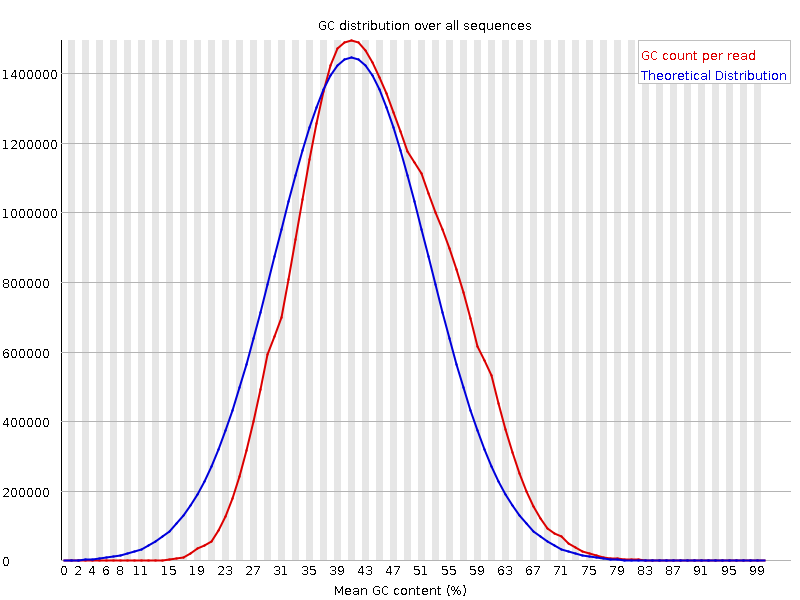
\includegraphics[width=0.9\linewidth]{../Figures/Ot729_index7_Exome_Sergio.Pena_RDNP_07262011-reads1-110716_I123_FCC043NABXX_L2_index7_1_fastqc/Images/per_sequence_gc_content.png}}
  \caption{Sequências Forward}
\end{subfigure}%
\begin{subfigure}{.7\textwidth}
  \centering
  \fbox{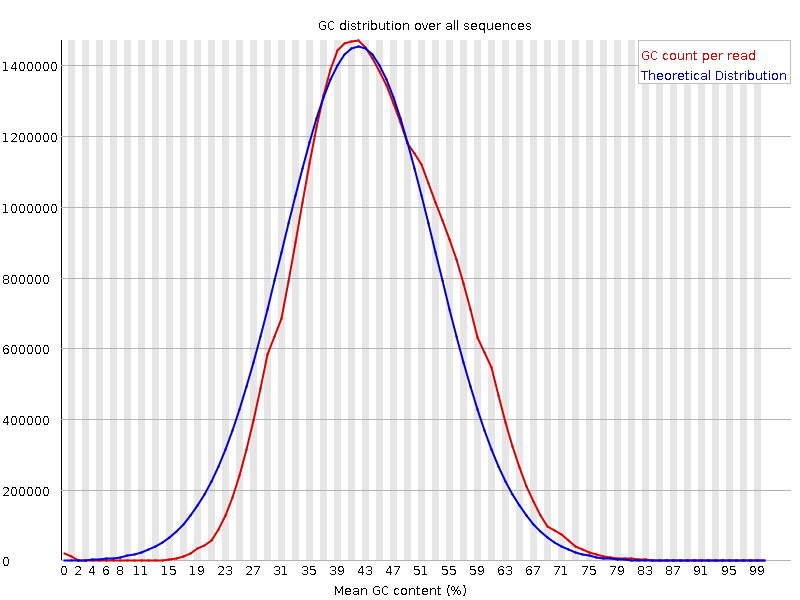
\includegraphics[width=0.9\linewidth]{../Figures/Ot729_index7_Exome_Sergio.Pena_RDNP_07262011-reads2-110716_I123_FCC043NABXX_L2_index7_2_fastqc/Images/per_sequence_gc_content.png}}
  \caption{Sequências Reverse}
\end{subfigure}
\caption[Distribuição do conteúdo de GC nas leituras]{Nesta figura podemos observar a distribuição do conteúdo GC ao longo das leituras.}
\label{fig:gc_content_per_sequence}
\end{figure}

\begin{figure}
\centering
\Large\textbf{Níveis de duplicação}\par\medskip
\begin{subfigure}{.7\textwidth}
  \centering
  \fbox{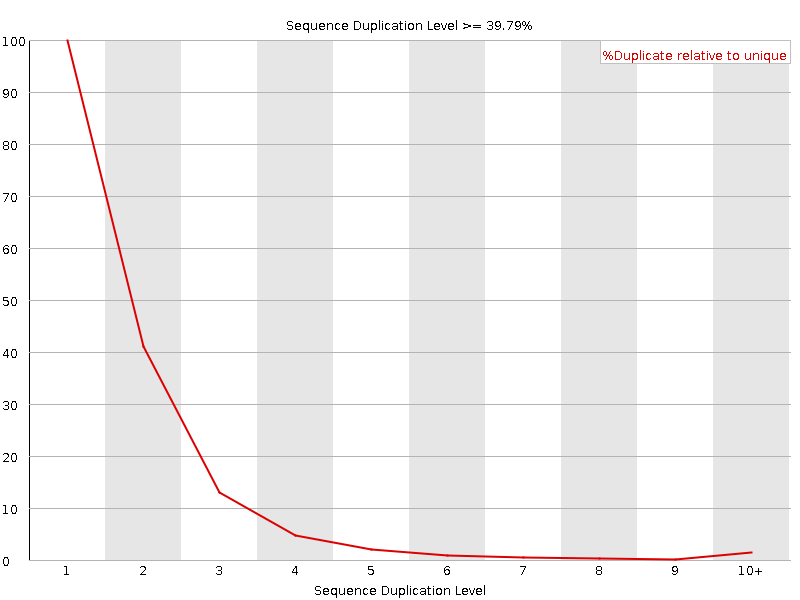
\includegraphics[width=0.9\linewidth]{../Figures/Ot729_index7_Exome_Sergio.Pena_RDNP_07262011-reads1-110716_I123_FCC043NABXX_L2_index7_1_fastqc/Images/duplication_levels.png}}
  \caption{Sequências Forward}
\end{subfigure}%
\begin{subfigure}{.7\textwidth}
  \centering
  \fbox{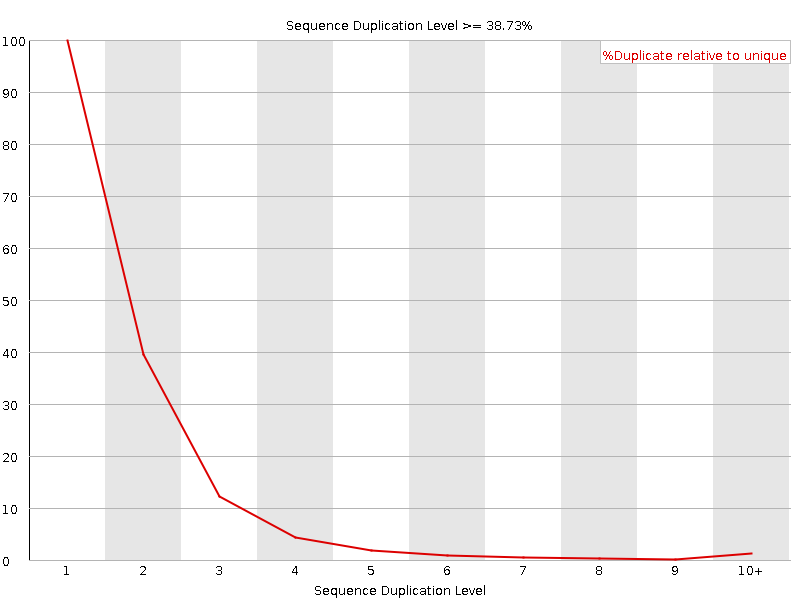
\includegraphics[width=0.9\linewidth]{../Figures/Ot729_index7_Exome_Sergio.Pena_RDNP_07262011-reads2-110716_I123_FCC043NABXX_L2_index7_2_fastqc/Images/duplication_levels.png}}
  \caption{Sequências Reverse}
\end{subfigure}
\caption[Níveis de duplicação]{Nesta figura podemos obersar os níveis de duplicação. Uma quantidade alta do nível de duplicação pode indicar um problema com o sequenciamento.}
\label{fig:duplication_levels}
\end{figure}

\begin{figure}
\centering
\Large\textbf{Perfis de K-mer}\par\medskip
\begin{subfigure}{.7\textwidth}
  \centering
  \fbox{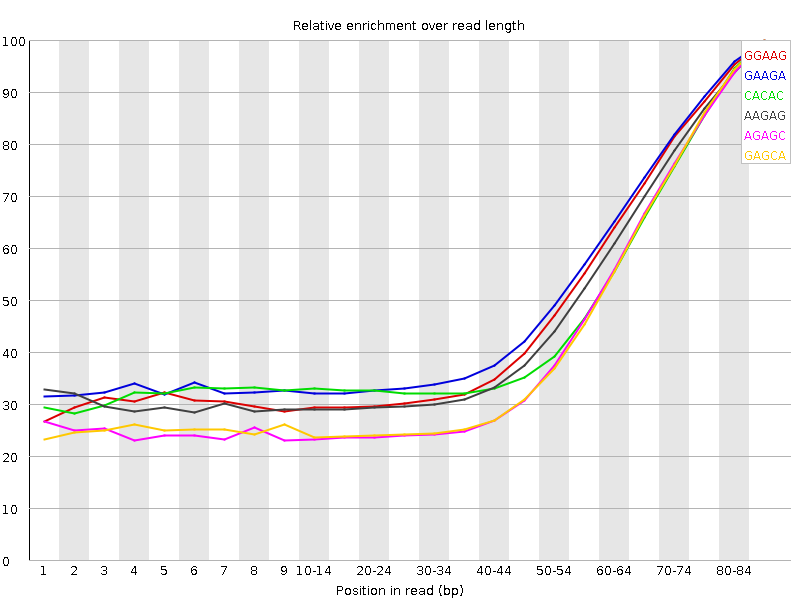
\includegraphics[width=0.9\linewidth]{../Figures/Ot729_index7_Exome_Sergio.Pena_RDNP_07262011-reads1-110716_I123_FCC043NABXX_L2_index7_1_fastqc/Images/kmer_profiles.png}}
  \caption{Sequências Forward}
\end{subfigure}%
\begin{subfigure}{.7\textwidth}
  \centering
  \fbox{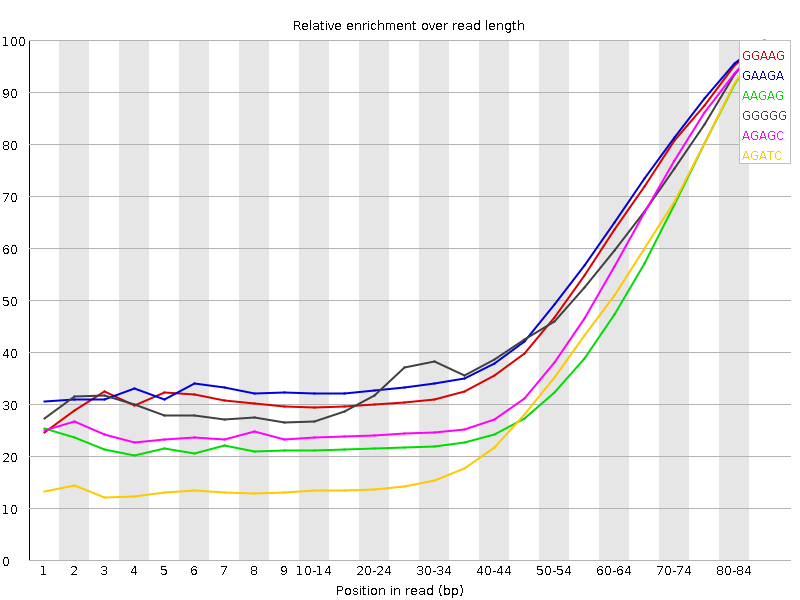
\includegraphics[width=0.9\linewidth]{../Figures/Ot729_index7_Exome_Sergio.Pena_RDNP_07262011-reads2-110716_I123_FCC043NABXX_L2_index7_2_fastqc/Images/kmer_profiles.png}}
  \caption{Sequências Reverse}
\end{subfigure}
\caption[Perfis de K-mer]{Nesta figura podemos observar o enriquecimento relativo do número de kmers ao longo das leituras, um desbalanceamento grande de um kmer específico pode indicar um problema com o sequenciamento.}
\label{fig:kmer_profiles}
\end{figure}

\end{landscape}

}

Antes de realizar o alinhamento foi necessário converter o escore de codificação das sequências do formato Illumina 1.5 para o formato Sanger utilizando um script em perl fornecido pelo programa MAQ (\url{http://maq.sourceforge.net/fq_all2std.pl}). Esta conversão é necessária para a análise dos dados utilizando o GATK.

\subsection{Alinhamento}

Após verificação da qualidade dos dados recebidos, foi feito um alinhamento utilizando o alinhador BWA que mapeou as leituras contra a versão b37 do genoma humano de referência.

Ao final deste mapeamento foi obtido um arquivo BAM como resultado e então foram extraídas métricas de qualidade sobre este alinhamento com o programa samstat. Este programa foi útil para ajudar a verificar métricas sobre a qualidade do alinhamento em arquivos do tipo BAM antes e depois de utilizarmos o GATK para melhorar a qualidade e corrigir alguns problemas nesses arquivos.

A seguir é apresentado um resumo do que aconteceu com os dados durante a execução do GATK dentro do pipeline de análise de exomas desenvolvido por este trabalho e apresentado na figura \ref{fig:exome_pipeline} na parte de Métodos.

\subsection{GATK Genome Analysis ToolKit}

Após o alinhamento com o BWA nós utilizamos o programa GATK para melhorar a qualidade das leituras e realizar o processo chamado de \textit{``calling das variantes''}. Para calcular a cobertura média do exoma, foi utilizado o programa bedtools \footnote{\url{https://github.com/arq5x/bedtools}} que procura por regiões definidas pelo kit de sequenciamento utilizado. O arquivo BED com os targets para este exoma foram obtidos no link: \href{http://www.nimblegen.com/products/seqcap/ez/v2/}{http://www.nimblegen.com/products/seqcap/ez/v2/}

Nas figuras~\ref{fig:rms_before_gatkv1} e~\ref{fig:rms_before_gatkv2} podemos observar um sumário sobre a qualidade do alinhamento das leituras antes de utilizarmos o GATK. Tivemos aproximadamente 71.4 milhões de leituras mapeadas e além disso 75\% dessas leituras tiveram um escore de alinhamento MAPQ acima de 30 o que pode ser considerado um resultado muito bom para este tipo de análise.

Nas figuras~\ref{fig:rms_after_gatkv1} e~\ref{fig:rms_after_gatkv2} apresentamos um sumário sobre o alinhamento depois que o GATK foi utilizado. Embora o número de leituras tenha diminuído em relação a figura anterior, nota-se um aumento no valor da qualidade na região final das leituras presentes.

\afterpage{
\begin{figure}[p]
\centering
\Large\textbf{Estatísticas do alinhamento antes de utilizarmos o GATK}\par\medskip
\fbox{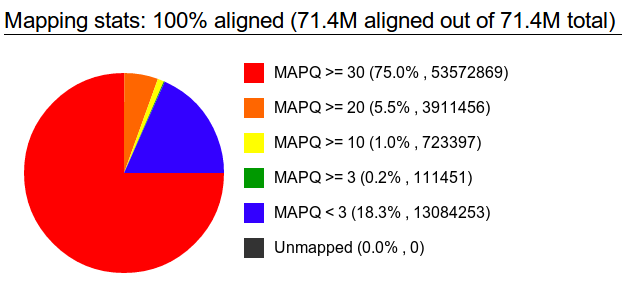
\includegraphics[width=0.9\textwidth]{alinhamento_rms/antes_gatk_summary.png}}
\caption[Estatísticas do alinhamento antes de utilizarmos o GATK]{Nesta figura podemos observar que o alinhamento obteve mais de 75\% das leituras com escore de phred maior do que 30.} \label{fig:rms_before_gatkv1}

\Large\textbf{Qualidade média por base do alinhamento antes de utilizarmos o GATK}\par\medskip
\fbox{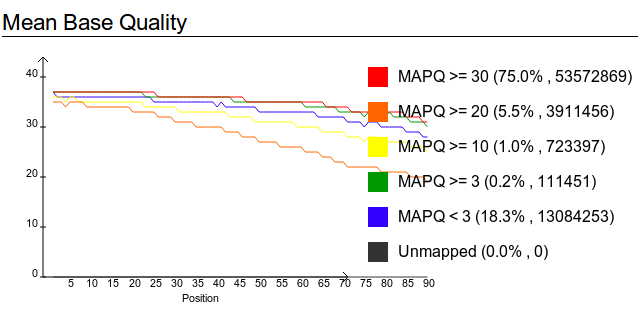
\includegraphics[width=0.9\textwidth]{alinhamento_rms/antes_gatk_mean_base_quality.png}}
\caption[Qualidade média por base do alinhamento antes de utilizarmos o GATK]{Nesta figura podemos observar a distribuição da qualidade ao longo das bases para cada grupo de leituras do alinhamento.} \label{fig:rms_before_gatkv2}
\end{figure}
\clearpage
}

\afterpage{
\begin{figure}[p]
\centering
\Large\textbf{Estatísticas do alinhamento depois de utilizarmos o GATK}\par\medskip
\fbox{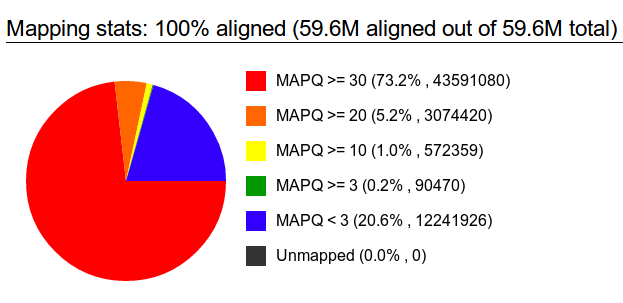
\includegraphics[width=0.9\textwidth]{alinhamento_rms/rms_after_gatk_mapping_stats.png}}
\caption[Estatísticas do alinhamento depois de utilizarmos o GATK]{Nesta figura podemos observar uma redução do número total de leituras devido a remoção de leituras com baixa qualidade dentro de cada um dos grupos.} \label{fig:rms_after_gatkv1}

\Large\textbf{Qualidade média por base do alinhamento depois de utilizarmos o GATK}\par\medskip
\fbox{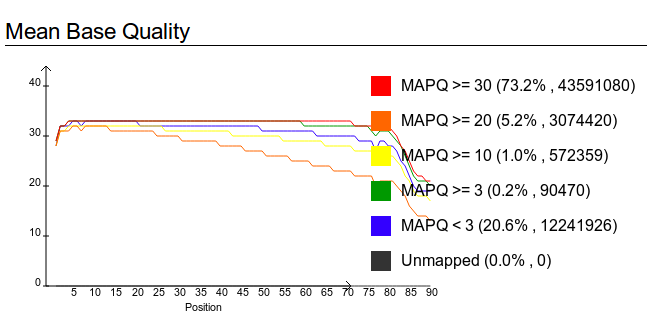
\includegraphics[width=0.9\textwidth]{alinhamento_rms/rms_after_gatk_mean_base_quality.png}}
\caption[Qualidade média por base do alinhamento depois de utilizarmos o GATK]{Nesta figura podemos observar uma estratificação maior da qualidade das leituras após a filtragem das leituras com baixa qualidade.} \label{fig:rms_after_gatkv2}
\end{figure}
\clearpage
}

\subsubsection{Remoção de leituras duplicadas}

Primeiro foi utilizado o comando MarkDuplicates para remover leituras duplicadas em nosso arquivo de alinhamento, durante este processo 17\% das leituras foram consideradas duplicadas e foram descartadas. Este passo é importante pois ajuda a reduzir os erros na hora de realizarmos o \textit{``calling das variantes''}. Esta remoção não diminui a cobertura do sequenciamento mas ajuda a melhorar a qualidade das áreas que foram cobertas. Ao final restaram 59.570.255 milhões de leituras passaram para a próxima etapa.

Na tabela \ref{aln_after_dedup} apresentamos um resumo detalhado das leituras contidas no arquivo de alinhamento após este processo.

\afterpage{
\begin{table}[p]
\caption{Informações sobre o alinhamento após a remoção de leituras duplicadas}
\begin{center}
\begin{tabular}{|l|l|}
\hline
no total (leituras que passaram no controle de qualidade) & 59.570.255 \\ \hline
mapeadas (84.31\% do total) & 50.222.733 \\ \hline
pareadas no sequenciamento & 59.570.255 \\ \hline
leitura1 & 29.756.446 \\ \hline
leitura2 & 29.813.809 \\ \hline
corretamente pareadas (80.78\%) & 48.122.446 \\ \hline
com ela própria e com a companheira mapeada & 49.778.115 \\ \hline
únicas (0.75\%) & 444.618 \\ \hline
com a leitura companheira mapeada em um cromossomo diferente & 112.890 \\ \hline
com a leitura companheira mapeada em um cromossomo diferente (mapQ>=5) & 66.095 \\ \hline
\end{tabular}
\end{center}
\label{aln_after_dedup}
\end{table}
\clearpage
}

\subsubsection{Realinhamento Local em regiões de Indels}

\subsubsubsection{Criação dos alvos para realinhamento}

Este método realiza uma busca ao longo do alinhamento por regiões que possuam características específicas como SNPs presentes no final das leituras que sejam discordantes para as leituras \textit{forward} e \textit{reverse} ou que estejam em regiões com repetição de nucleotídeos, por exemplo (TTTTT). Então, ele marca estas regiões para que um realinhamento local seja realizado utilizando o método de Smith–Watermann com o objetivo de corrigir possíveis erros gerados durante o alinhamento dessas sequências e encontrar indels nesta região.

A seguir apresentamos o resultado da saída deste método:

\begin{itemize}
  \item Tempo de execução 5719.67 segundos, 95.33 minutos, 1.59 horas.
  \item 3.611.533 leituras foram filtradas durante o processo de um total de 51.194.954 (7,05 \%).
  \item 3.611.499 leituras (7.05\% do total) falharam o filtro de qualidade zero de mapeamento.
  \item 34 leituras (0.00\% do total) falharam o filtro de leituras não mapeadas.
\end{itemize}


\subsubsubsection{Aplicação da Recalibração}

Este método realiza um realinhamento local nas leituras selecionadas pelo passo anterior para tentar melhorar a posição das leituras em relação a regiões com indels. Por exemplo, quando temos uma indel verdadeira que foi mapeada contra o genoma de referência, as leituras próximas a essa indel estarão mapeadas incorretamente se a região de início ou fim da leitura estiver próxima ao indel.

Após este processo o comando FixMate do programa Picard foi utilizado para remover as leituras órfãs, ou seja aquelas que o seu par tenha sido descartado durante este processo.

\subsubsection{Recalibração do Escore de Qualidade da Base}

Após o realinhamento de indels o GATK possui uma etapa de recalibração dos escores de qualidade. Este processo avalia a maneira como cada leitura varia em relação as outras leituras com o objetivo de deixar os valores mais uniformes e corrigir um possível viés de cada tecnologia.

A seguir apresentamos gráficos mostrando o que acontece com os dados antes e depois deste processo.

\afterpage{
\begin{landscape}

\begin{figure}
\centering
\Large\textbf{Escore de Qualidade Empírico vs Reportado}\par\medskip
\begin{subfigure}{.7\textwidth}
  \centering
  \fbox{\includegraphics[width=0.9\linewidth]{alinhamento_rms/exome.sorted.dedup.real.fixed.recal.stats.before/emp_v_stated.pdf}}
  \caption{Antes da recalibração do escore de qualidade}
\end{subfigure}%
\begin{subfigure}{.7\textwidth}
  \centering
  \fbox{\includegraphics[width=0.9\linewidth]{alinhamento_rms/exome.sorted.dedup.real.fixed.recal.stats.after/emp_v_stated.pdf}}
  \caption{Depois da recalibração do escore de qualidade}
\end{subfigure}
\caption[Escore de Qualidade Empírico vs Reportado]{Nesta figura podemos observar uma estratificação maior do escore de qualidade, este processo ajudar a corrigir um viés que existe no escore de qualidade de acordo com cada plataforma.}
\label{fig:rms_before_emp_v_stated}
\end{figure}

\begin{figure}
\centering
\Large\textbf{Número de Bases vs Escore de Qualidade}\par\medskip
\begin{subfigure}{.7\textwidth}
  \centering
  \fbox{\includegraphics[width=0.9\linewidth]{alinhamento_rms/exome.sorted.dedup.real.fixed.recal.stats.before/quality_rep_hist.pdf}}
  \caption{Antes da recalibração do escore de qualidade}
\end{subfigure}%
\begin{subfigure}{.7\textwidth}
  \centering
  \fbox{\includegraphics[width=0.9\linewidth]{alinhamento_rms/exome.sorted.dedup.real.fixed.recal.stats.after/quality_rep_hist.pdf}}
  \caption{Depois da recalibração do escore de qualidade}
\end{subfigure}
\caption[Número de Bases vs Escore de Qualidade]{Nessa figura podemos observar uma distribuição maior do valor médio do escore de qualidade.}
\label{fig:rms_quality_rep_hist}
\end{figure}

\begin{figure}
\centering
\Large\textbf{Qualidade (Empírico - Reportado) vs Dinucleotídeos}\par\medskip
\begin{subfigure}{.7\textwidth}
  \centering
  \fbox{\includegraphics[width=0.9\linewidth]{alinhamento_rms/exome.sorted.dedup.real.fixed.recal.stats.before/qual_diff_v_Dinuc.pdf}}
  \caption{Antes da recalibração do escore de qualidade}
\end{subfigure}%
\begin{subfigure}{.7\textwidth}
  \centering
  \fbox{\includegraphics[width=0.9\linewidth]{alinhamento_rms/exome.sorted.dedup.real.fixed.recal.stats.after/qual_diff_v_Dinuc.pdf}}
  \caption{Depois da recalibração do escore de qualidade}
\end{subfigure}
\caption[Qualidade (Empírico - Reportado) vs Dinucleotídeos]{Nesta figura podemos observar uma correção da qualidade para cada dinucleotídeo.}
\label{fig:rms_qual_diff_v_Dinuc}
\end{figure}

\end{landscape}

}


Na figura \ref{fig:rms_before_emp_v_stated} apresentamos o antes e o depois para os valores de qualidade empíricos contra os valores reais estimados. Podemos notar que este método realiza uma normalização dos dados de maneira a corrigir um viés existente por causa das particularidades de cada tecnologia de sequenciamento.

Na figura \ref{fig:rms_quality_rep_hist} apresentamos a relação entre o número de bases e os valores de qualidade em phred escore. Neste gráfico podemos observar que a maior parte das bases estão com um phred escore entre 30 e 40 o que pode ser considerado um resultado muito bom.

Na figura \ref{fig:rms_qual_diff_v_Dinuc} podemos notar um viés da relação entre a qualidade empírica e reportada para diferentes tipos de dinucleotídeos. Neste processo os valores são normalizados ao redor de 0, para ajudar a reduzir o número de falsos positivos no processo seguinte de calling de variantes.

\subsubsection{Chamada de variantes}

O processo de chamada ``\textit{calling}'' de variantes foi realizado com o método UnifiedGenotyper do GATK considerado o padrão ouro atualmente para se fazer esse tipo de tarefa.

A tabela \ref{rms_calling} apresenta um resumo dos resultados obtidos neste processo:

\afterpage{
\begin{landscape}

\begin{table}[p]
\caption{Resultado do processo de calling de variantes realizado usando o método UnifiedGenotyper para o indivíduo RMS}
\begin{center}
\scalebox{1.5}{
\begin{tabular}{|r|l|}
\hline
Bases visitadas & 47.195.691 \\ \hline
Bases que podem ser chamadas & 46.982.901 \\ \hline
Bases chamadas com confiança & 827.992 \\ \hline
\% de bases que podem ser chamadas de todas as regiões & 99,549 \\ \hline
\% de bases que podem ser chamadas com confiança de todas as regiões & 1,754 \\ \hline
\% de bases chamadas com confiança de todas as regiões & 1,762 \\ \hline
Chamadas realmente feitas (variantes realmente encontradas) & 39.677 \\ \hline
\end{tabular}
}
\end{center}
\label{rms_calling}
\end{table}
\end{landscape}

\clearpage
}

Podemos observar que tivemos um \textit{calling} de 39.677 variantes em 47.195.691 bases visitadas no total, o que corresponde a 1.75\% do genoma. De todas as bases cobertas 827.992 puderam ser genotipadas com um grau de confiança de 99.5\%. A cobertura média desse exoma foi de 29.96X e o valor do escore de qualidade médio foi de 504.62.

\subsubsection{Recalibração do Escore de Qualidade da Variante}

Neste processo nós utilizamos um conjunto de dados com genótipos dos indivíduos do projeto HapMap 3 que foram validados utilizando arrays de SNPs e com isso criamos um modelo de treinamento sobre esses atributos. Este modelo é então aplicado no arquivo VCF para melhorar a qualidade das variantes obtidas e ajudar a reduzir o número de falsos positivos.

\subsubsection{Processo de Filtragem de Indels}

Este processo consiste na aplicação de alguns critérios de filtragem para eliminar indels de baixa qualidade, como por exemplo: 

\begin{itemize}
 \item QD < 2.0
 \item ReadPosRankSum < -20.0
 \item InbreedingCoeff < -0.8
 \item FS > 200.0 
\end{itemize}

Esses valores foram obtidos a partir do site do GATK em seu documento sobre ``\textit{Best Practices for Variant Detection}''

Site: \url{https://www.broadinstitute.org/gatk/guide/best-practices}

\section{Anotação de Exomas}

Após a obtenção do arquivo VCF final gerado pelo programa GATK, um script em python realiza a anotação dos dados utilizando os programas SNPEFF, Variant Annotator (GATK) e o Annovar integrando os resultados de cada um dos programas em um único arquivo VCF final. Após obtermos os resultados da anotação surgiu a ideia de construir uma ferramenta online que permitisse a filtragem das variantes por médicos e cientistas, de maneira que esta operação pudesse ser realizada através de uma interface web que permitisse a identificação de variantes que pudessem estar associadas com a doença.

\section{Mendel,MD - Construção da Ferramenta}

A seguir apresentamos o software Mendel,MD, que foi desenvolvido para investigação dos casos clínicos recebidos pelo Laboratório de Genômica Clínica da Faculdade de Medicina da UFMG. Esse programa foi criado para permitir o armazenamento, a anotação e a filtragem de variantes dos pacientes que foram estudados pelo nosso grupo, com a ideia de criar uma maneira fácil de atualizar os dados rapidamente, toda vez que novos conjuntos de dados, programas ou métodos fossem disponibilizados, de forma simples e modular, facilitando ao máximo a repetição das tarefas que fossem comuns. Este \textit{pipeline} pode ser facilmente adaptado ou modificado para inclusão de novos métodos e novas ferramentas.

\subsection{Banco de Dados}
A modelagem do banco de dados foi feita através de um arquivo chamado \textit{models.py} que possui classes em python que descrevem os campos que devem ser armazenados em cada uma das tabela do banco de dados. Após a criação deste arquivo, o Django passa então a controlar os processos de criação e atualização desses campos. Além disso ele também fica responsável pela busca e remoção dos dados através uma técnica conhecida como Mapeamento de Objetos Relacionais (ORM) que facilita a criação de consultas em Python que são transformadas em SQL para se realizar consultas ao banco de dados. Isso é muito utilizado para filtrar as variantes de cada paciente de acordo com os parâmetros que forem escolhidos pelo médico ou pesquisador que estiver utilizando o Mendel,MD.

No anexo~\ref{lst:modelo_individuo} apresentamos o modelo que foi desenvolvido para armazenar as informações sobre cada individuo. Neste arquivo ficam armazenadas informações como por exemplo o nome de usuário que fez o upload do arquivo VCF, a data do upload, o nome completo do arquivo e algumas informações sobre o estado do arquivo dentro do sistema.

Após ser inserido no Mendel,MD, o arquivo VCF passa a ter três estados possíveis dentro do sistema: \textit{new}, \textit{annotated} e \textit{populated}. O estado \textit{new} indica que o arquivo acabou de ser enviado ao sistema e está na fila para ser anotado pelo nosso programa, o estado \textit{annotated} significa que ele passou por todo o \textit{pipeline} de anotação com sucesso e está pronto na fila para ser inserido no banco de dados e o estado \textit{populated} indica que ele já foi inserido no banco de dados com sucesso e está pronto para ser analisado pelo usuário final.

No anexo~\ref{lst:modelo_variantes} apresentamos o modelo que foi desenvolvido para armazenar as informações sobre as variantes de cada indivíduo. Podemos observar que além dos campos já presentes no VCF, foram criados alguns campos para ajudar na filtragem de variantes como por exemplo a frequência da variante em relação a diferentes bancos de dados (ex. 1000genomesn, dbSNP e ESP6500) e alguns escores de patogenicidade como por exemplo SIFT e Polyphen-2 e CADD. Também podemos observar que alguns campos foram criados para armazenar as informações de duas ferramentas que foram integradas no sistema SnpEff e VEP.

Para recuperarmos a partir do banco todas as variantes do primeiro indivíduo do nosso banco de dados usamos o seguinte código em Python (Django):

\begin{verbatim}
Variants.objects.all(individual_id=1)
\end{verbatim}

Se quisermos obter todas as variantes desse indivíduo que são homozigóticas nós usamos o seguinte código:

\begin{verbatim}
Variants.objects.all(individual_id=1, variant_type="HOM")
\end{verbatim}

Essa codificação dos campos em Python permite que eles sejam facilmente traduzidos para um código SQL compatível com o sistema gerenciador de banco de dados (SGBD) que estiver sendo utilizado pelo projeto, que no nosso caso é o banco PostgreSQL.

Os dados deste trabalho foram inicialmente armazenados em um banco MySQL e posteriormente migrados para um banco PostgreSQL. Isso aconteceu porque o número de registros armazenados na tabela de variantes ultrapassou 10 milhões e a consulta ao banco de dados começou a ficar muito lenta, por exemplo, quando muitos indivíduos fossem utilizados como controles durante o processo de análise e filtragem de variantes. Após a migração do banco nós obtivemos um aumento de desempenho considerável que ajudou a melhorar bastante a usabilidade do sistema.

Na tabela \ref{table:registros} nós apresentamos informações sobre o número de registros armazenados em cada uma das tabelas do banco de dados. Aqui é possível visualizar o número de indivíduos, genes, doenças e vias metabólicas que foram armazenados em cada uma das tabelas do banco. Esses dados são muito importantes para auxiliarem na filtragem de variantes de cada indivíduo.



\afterpage{
\begin{table}[p]
\caption{Informação sobre o número de registros armazenados em cada uma tabelas do sistema.}
\begin{center}
\scalebox{0.65}{
\begin{tabular}{|p{6cm}|p{2cm}|p{10cm}|p{3cm}|}
\hline
\textbf{Tabela} & \textbf{número de registros} & \textbf{Tabela} & \textbf{número de registros} \\ \hline
account\_emailaddress         & 8                  & djkombu\_queue                                & 3                  \\ \hline
account\_emailconfirmation    & 8                  & filter\_analysis\_familyfilteranalysis        & 0                  \\ \hline
auth\_group                   & 0                  & filter\_analysis\_filteranalysis              & 0                  \\ \hline
auth\_group\_permissions      & 0                  & filter\_analysis\_filterconfig                & 0                  \\ \hline
auth\_permission              & 150                & genes\_cgdcondition                           & 3.607               \\ \hline
auth\_user                    & 12                 & genes\_cgdentry                               & 2.725               \\ \hline
auth\_user\_groups            & 0                  & genes\_cgdentry\_CONDITIONS                   & 3.958               \\ \hline
auth\_user\_user\_permissions & 0                  & genes\_cgdentry\_INTERVENTION\_CATEGORIES     & 3.635               \\ \hline
cases\_case                   & 0                  & genes\_cgdentry\_MANIFESTATION\_CATEGORIES    & 7.319               \\ \hline
cases\_case\_case\_groups     & 0                  & \textbf{genes\_gene}                          & \textbf{37.215}     \\ \hline
cases\_case\_cases            & 0                  & genes\_gene\_diseases                         & 5.725               \\ \hline
cases\_case\_children         & 0                  & genes\_genecategory                           & 0                  \\ \hline
cases\_case\_control\_groups  & 0                  & genes\_genecategory\_genes                    & 0                  \\ \hline
cases\_case\_controls         & 0                  & genes\_genegroup                              & 0                  \\ \hline
cases\_case\_shared\_with     & 0                  & genes\_genelist                               & 62                 \\ \hline
celery\_taskmeta              & 712                & genes\_goterm                                 & 0                  \\ \hline
celery\_tasksetmeta           & 0                  & genes\_goterm\_children                       & 0                  \\ \hline
databases\_varisnp            & 78.951 & genes\_goterm\_parents                        & 0                  \\ \hline
\textbf{diseases\_disease}    & \textbf{6.845}     & genes\_intervention                           & 20                 \\ \hline
diseases\_gene                & 4.715              & genes\_manifestation                          & 19                 \\ \hline
diseases\_gene\_diseases      & 6.845              & genes\_membership                             & 0                  \\ \hline
diseases\_hgmdgene            & 0                  & individuals\_controlgroup                     & 0                  \\ \hline
diseases\_hgmdgene\_diseases  & 0                  & individuals\_controlvariant                   & 0                  \\ \hline
diseases\_hgmdmutation        & 0                  & individuals\_group                            & 3                  \\ \hline
diseases\_hgmdphenotype       & 0                  & individuals\_group\_members                   & 76                 \\ \hline
django\_admin\_log            & 2                  & \textbf{individuals\_individual}              & \textbf{221}       \\ \hline
django\_content\_type         & 50                 & individuals\_individual\_shared\_with\_groups & 179                \\ \hline
django\_select2\_keymap       & 0                  & individuals\_individual\_shared\_with\_users  & 0                  \\ \hline
django\_session               & 511                & individuals\_usergroup                        & 1                  \\ \hline
django\_site                  & 1                  & individuals\_usergroup\_members               & 2                  \\ \hline
djcelery\_crontabschedule     & 0                  & pathway\_analysis\_pathway                    & 289                \\ \hline
djcelery\_intervalschedule    & 0                  & socialaccount\_socialaccount                  & 0                  \\ \hline
djcelery\_periodictask        & 0                  & socialaccount\_socialapp                      & 0                  \\ \hline
djcelery\_periodictasks       & 0                  & socialaccount\_socialapp\_sites               & 0                  \\ \hline
djcelery\_taskstate           & 0                  & socialaccount\_socialtoken                    & 0                  \\ \hline
djcelery\_workerstate         & 0                  & \textbf{variants\_variant}                    & \textbf{25.304.952}  \\ \hline
djkombu\_message              & 0                  &                                               &                    \\ \hline
\end{tabular}
}
\end{center}
\label{table:registros}
\end{table}
\clearpage
}

\normalsize

Atualmente o nosso banco de dados possui 221 exomas e isso equivale a 25.304.952 variantes.

\subsection{Dashboard}

Para facilitar a visualização dos indivíduos no sistema foi desenvolvida uma interface chamada de \textit{Dashboard} que exibe uma lista com todos os arquivos que foram enviados para o sistema. Na figura \ref{fig:dashboard} apresentamos essa interface e podemos observar que com ela é possível verificar diversas informações sobre cada indivíduo como o nome de cada arquivo, o número de variantes, a data de envio, o estado atual do arquivo no sistema entre outras informações. Também nesta página é possível realizar operações em massa como por exemplo, selecionar múltiplos indivíduos através de uma caixa de seleção ao lado de cada indivíduo pra poder enviar os arquivos para serem re-anotados ou re-inseridos no banco de dados sempre quando for necessário. Este tipo de interface facilita muito a manipulação e anotação dos VCFs sempre que houver novas informações para serem integradas na análise de exomas.


\afterpage{
\begin{landscape}
\begin{figure}[p]
  \centering
    \Large\textbf{Dashboard - Interface para visualização dos indivíduos no sistema}\par\medskip
  \fbox{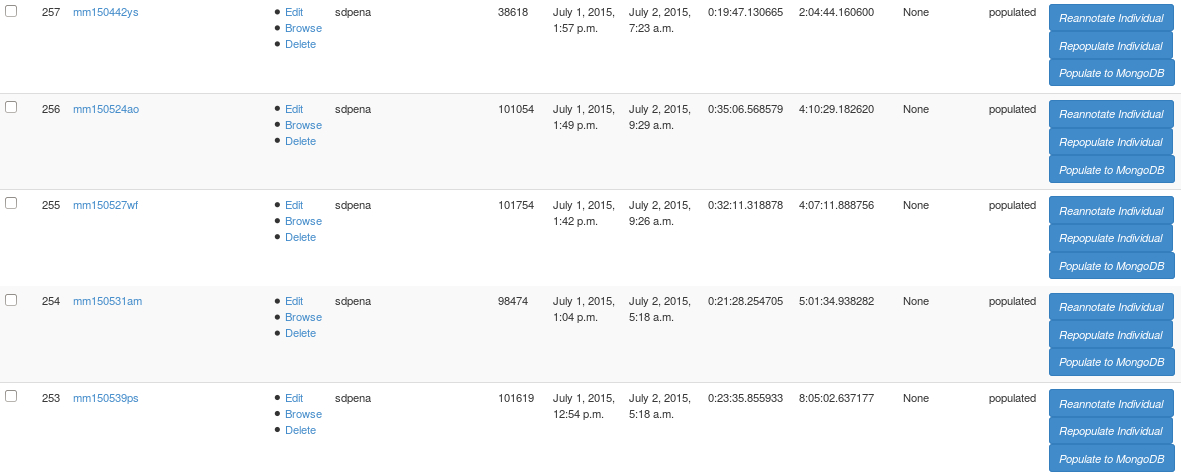
\includegraphics[width=1.3\textwidth]{./Figures/mendelmd/Dashboard.png}}
  \caption[Dashboard - Interface para visualização dos indivíduos no sistema]{A partir desta interface é possível visualizar as variantes de cada indivíduo, reanotar os indivíduos e reinserí-los no banco de dados. Da esquerda para a direita temos as colunas: ID, nome da amostra, usuário, número de variantes, Data da criação, data da modificação, tempo de anotação, tempo de inserção no banco de dados e estado da amostra.}
  \label{fig:dashboard}
\end{figure}
\end{landscape}

\clearpage
}


\subsection{Upload de Genomas}

A figura~\ref{fig:upload} apresenta a interface de submissão de indivíduos para o sistema. Essa interface foi desenvolvida utilizando a biblioteca de javascript chamada Jquery FileUpload e facilita o envio de arquivos VCFs para o sistema permitindo o upload simultâneo de indivíduos para o servidor usando para isso qualquer dispositivo (computador, tablet ou celular) que tenha acesso a internet.

\afterpage{
  \begin{landscape}
\begin{figure}[p]
  \centering
  \Large\textbf{Interface para submissão dos indivíduos no sistema}\par\medskip
  \fbox{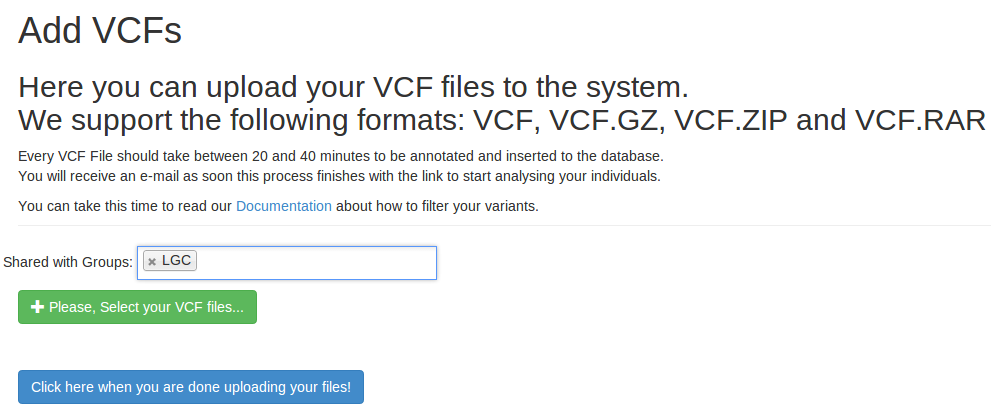
\includegraphics[width=1.5\textwidth]{./Figures/mendelmd/upload.png}}
  \caption[Interface para submissão dos indivíduos no sistema]{A interface de submissão dos indivíduos foi desenvolvida utilizando a biblioteca Jquery FileUpload para facilitar essa tarefa.}
  \label{fig:upload}
\end{figure}
\end{landscape}
\clearpage
}


\subsection{Agendador de Tarefas}

O Celery é um sistema agendador de tarefas assíncronas e distribuídas que permite a integração e execução de diferentes scripts e programas. Este programa foi utilizado para permitir a anotação automática dos dados de maneira totalmente assíncrona a partir do momento que o usuário realiza o upload dos dados no sistema. Nas figuras~\ref{fig:celery_shell} e~\ref{fig:celery_annotation} apresentamos a interface do celery, na figura ~\ref{fig:celery_annotation} é possível verificar diversos scripts sendo executados em paralelo para realizar a anotação de um exoma que foi inserido no sistema.

\afterpage{
  \begin{landscape}
\begin{figure}[p]
  \centering
  \Large\textbf{Interface do Celery}\par\medskip
    \fbox{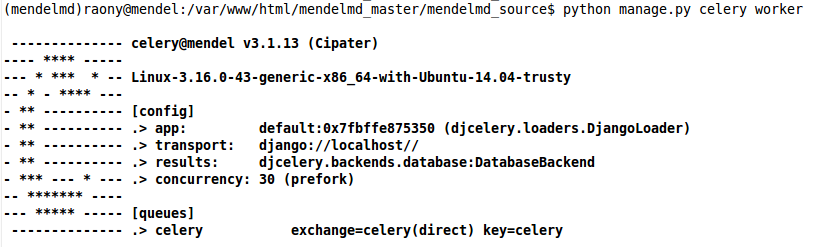
\includegraphics[width=1.5\textwidth]{./Figures/Celery_Shell.png}}
  \caption[Interface do Celery]{Nesta figura podemos visualizar a interface de comando do Celery. Nesta interface podemos verificar o output de cada programa utilizado durante a anotação de variantes.}
  \label{fig:celery_shell}
  \end{figure}
\end{landscape}

\clearpage
}


\afterpage{
  \begin{landscape}
\begin{figure}[p]
  \centering
  \Large\textbf{Processo de anotação de variantes}\par\medskip
  \fbox{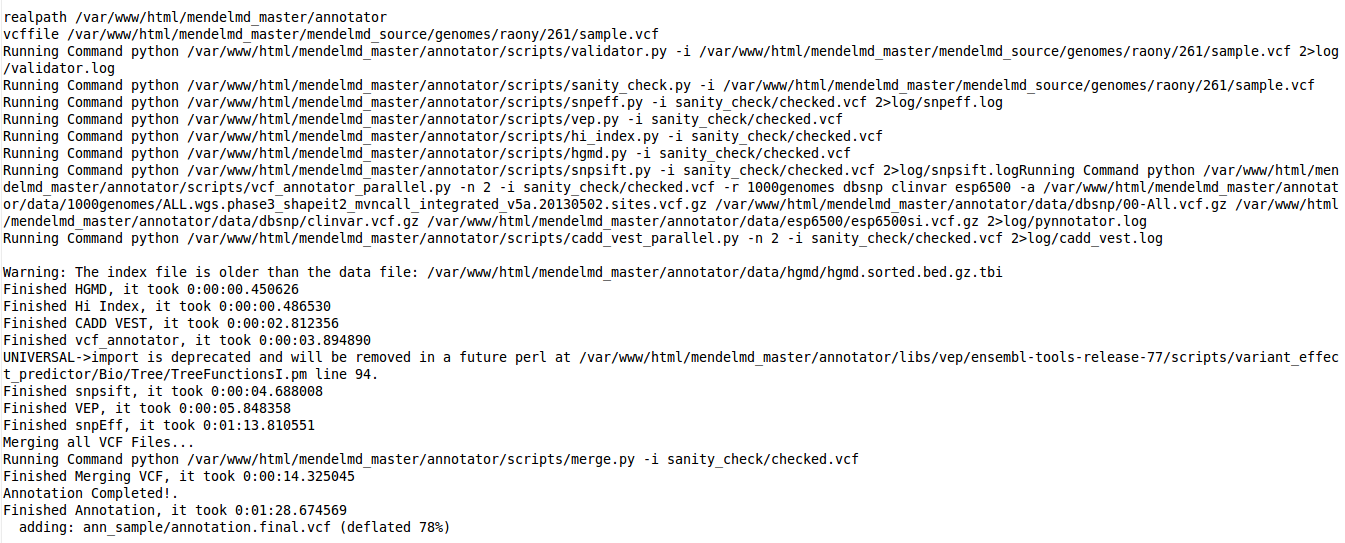
\includegraphics[width=1.5\textwidth]{./Figures/Celery_annotation.png}}
  \caption[Processo de anotação de variantes]{Nesta figura podemos observar diversos scripts sendo executados em paralelo utilizando o Celery para realizar a anotação de exomas através do uso de diferentes programas como SnpEff e VEP.}
  \label{fig:celery_annotation}
  \end{figure}
\end{landscape}

  
  \clearpage
}

\subsection{Conversão dos dados para CSV}

Apesar do Mendel,MD ter sido criado para facilitar o processo de filtragem dos dados utilizando para isso uma interface web, nós também desenvolvemos um script em python para realizar a conversão dos dados de VCF para CSV após o término do processo de anotação. Além disso foi desenvolvido uma programa usando wxPython que permite a conversão entre arquivos do tipo VCF para CSV de maneira local utilizando para isso uma interface gráfica com janelas e botões. Isso permite que o usuário converta os dados de VCF para CSV para que eles possam ser filtrados manualmente pelo Médico ou Pesquisador usando um programa de planilhas, como por exemplo o Excel ou o Libre Office Calc.

A figura~\ref{fig:vcf2csv} apresenta a interface gráfica desenvolvida para realizar essa conversão entre os formatos VCF e CSV. Essa transformação entre os formatos também realiza a de-normalização dos dados presentes nas colunas INFO do VCF de maneira que todos os dados dessa coluna fiquem separados em colunas diferentes no arquivo CSV final.

Além disso, também foi adicionada uma opção para que o usuário pudesse alterar a ordem das colunas no arquivo de saída.

\afterpage{
\begin{landscape}

\begin{figure}[p]
  \centering
  \Large\textbf{Programa desenvolvido para conversão entre arquivos VCF e CSV}\par\medskip
  \fbox{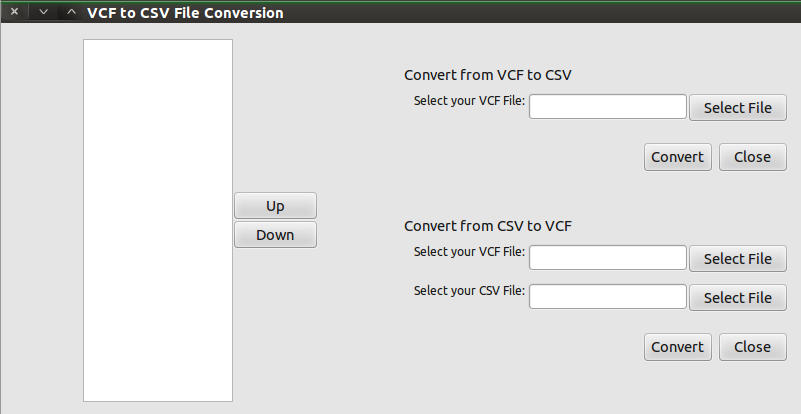
\includegraphics[width=1.5\textwidth]{./Figures/vcf2csv.png}}
  \caption[Programa desenvolvido para conversão entre arquivos VCF e CSV]{Interface do programa desenvolvido para conversão entre os formatos VCF e CSV.}
  \label{fig:vcf2csv}
\end{figure}
\end{landscape}
\clearpage
}

\subsection{Anotação de Variantes}

Para realizar a integração de diferentes ferramentas e fontes de informação, foi desenvolvido um \textit{framework} que realiza toda a anotação das variantes e que integra a maior parte dos dados e ferramentas existentes relacionados a este tipo de análise. A figura \ref{fig:framework_anotacao} é a principal figura deste trabalho, onde é apresentado o \textit{framework} que foi desenvolvido durante este trabalho. Pode-se observar nesta figura todos os processos que ocorrem dentro do pipeline de anotação desenvolvido para o Mendel,MD.

Após a inserção dos indivíduos no sistema, nós primeiramente realizamos uma validação dos arquivos VCFs através de um método chamado ``\textit{vcf-validator}'' que faz parte do programa \textit{VCFTools}. Este método realiza diversos testes no arquivo VCF de entrada e ao final gera um arquivo com todos os problemas que foram encontrados. Após essa validação inicial o arquivo passa então por um método que desenvolvemos chamado de ``\textit{sanity-check}'' que prepara o arquivo VCF para ser anotado por diferentes ferramentas.

Uma das primeiras ferramentas integradas para a anotação dos dados foi o SNPEFF que entre outras coisas fornece informações importantes sobre cada mutação como por exemplo a classificação do seu impacto de acordo com as seguintes classes: MODIFIER, LOW, MODERATE e HIGH. Essas classes são extremamente úteis na hora de realizarmos a filtragem de variantes, o mais recomendado aqui seria primeiro fazer a busca em variantes que são MODERATE e HIGH pois aí estarão presentes as mutações que são mais graves e possivelmente podem causar uma alteração da estrutura de uma proteína.

Outro programa integrado pela nossa anotação foi o Variant Effect Predictor (VEP). Este programa realiza a anotação das variantes em relação aos tipos de mutações encontradas, aos aminoácidos que estão alterados, e caso ela seja uma mutação não-sinônima, anota a posição em relação ao cDNA. Além disso, o VEP também fornece escores de patogenicidade como por exemplo o SIFT e o Polyphen2 que são os escores mais utilizados atualmente quando buscamos por variantes patogênicas.

O banco de dados dbNFSP trouxe a capacidade de agregar centenas de informações diferentes para nossa análise como por exemplo anotação em relação a diferentes bancos de dados, escores de patogenicidade e de conservação de mutações. Para integrar essa ferramenta nós desenvolvemos um script em python chamado de ``\textit{pynnotator}'' que por sua vez utiliza bibliotecas como \textit{pysam} e \textit{parallel python} para realizar a anotação dos dados de uma maneira rápida eficiente, inclusive fazendo o uso de  múltiplos cores do processador ao mesmo tempo. Esse tipo de implementação não foi trivial mas ajudou bastante a diminuir o tempo necessário para se realizar a anotação de cada VCF contra uma grande quantidade de dados. O tempo médio de anotação para cada exoma enviado para o sistema é de apenas dez minutos.

\afterpage{
\begin{landscape}

\begin{figure}[p]
  \centering
  \Large\textbf{Framework de anotação de variantes}\par\medskip
 \fbox{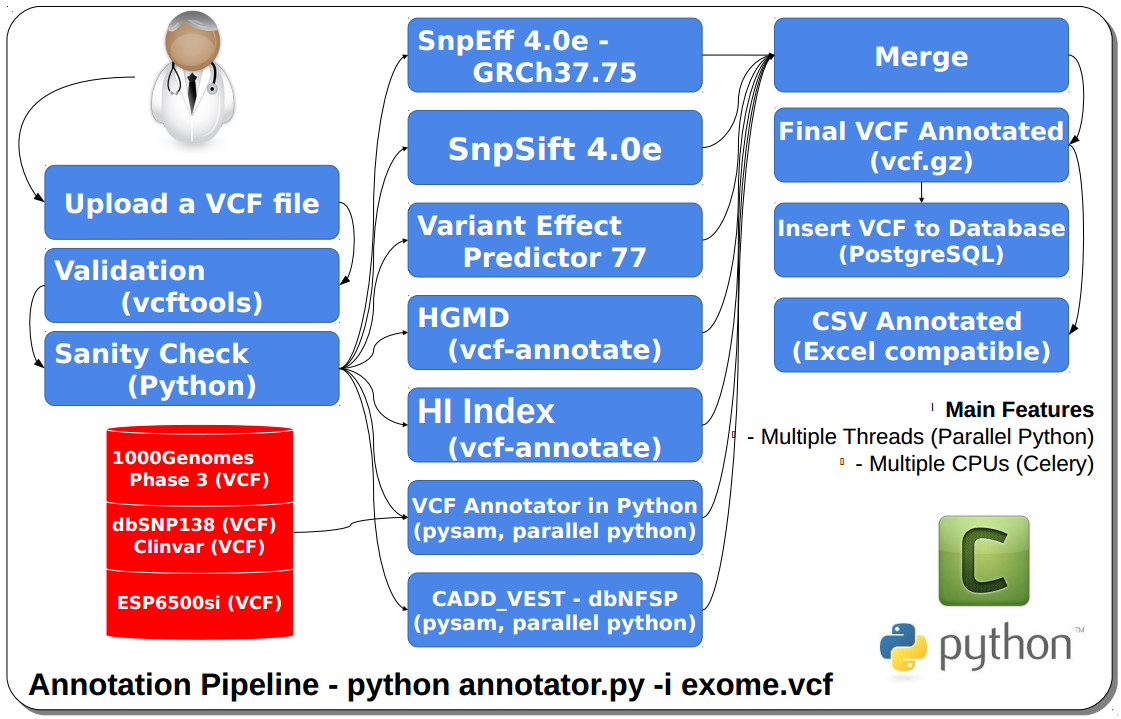
\includegraphics[width=1.2\textwidth]{./Figures/mendelmd/annotation_pipeline.png}}
 \caption[Framework de anotação de variantes]{Este foi o framework de anotação de variantes desenvolvido durante este trabalho, ele realiza a integração de diversas ferramentas e bancos de dados diferentes através de scripts desenvolvidos em python para automatizar todo o processo.}
 \label{fig:framework_anotacao}
\end{figure}
\end{landscape}

\clearpage
}

\subsection{Controle de Qualidade sobre os dados}

Para se realizar o controle de qualidade sobre os dados foi desenvolvida uma interface para calcular e mostrar métricas de qualidade calculadas a partir dos VCFs de cada indivíduo. Na figura \ref{fig:individuals_view} podemos observar algumas o número de variantes homozigotas e heterozigotas (0/1 e 1/1). Além disso nesta seção é possivel verificar outras métricas como o número de variantes para cada indivíduo, a cobertura média de cada exoma, a qualidade média de suas variantes, o número de variantes por cromossomo, o número de variantes por classe funcional entre outras opções que são apresentadas.

\afterpage{
    \begin{landscape}
\begin{figure}[p]
  \centering
    \Large\textbf{Interface para visualizar métricas sobre os dados inseridos}\par\medskip
   \fbox{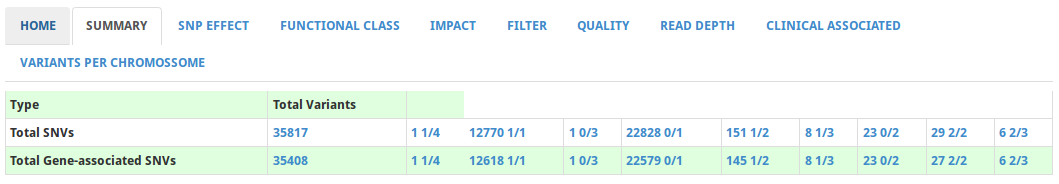
\includegraphics[width=1.5\textwidth]{./Figures/mendelmd/individuals_view.png}}
  \caption[Interface para visualizar métricas sobre os dados inseridos]{Nesta interface podes visualizar o número total de variantes, os tipos de variante encontradas no indivíduo e diversas outras métricas que são importantes para auxiliarem na filtragem de variantes como o número médio de qualidade e de cobertura para cada indivíduo.}
  \label{fig:individuals_view}
    \end{figure}
\end{landscape}


\clearpage
}

\subsection{Genes}

Na figura \ref{fig:genes_search} apresentamos a interface desenvolvida para realizar a busca de genes no sistema. Com essa interface é possível buscar genes por ``gene symbol'', por exemplo ``\textit{SUCLA2}'' ou então por uma parte do nome do gene ``succinate'' e então selecionar os genes obtidos nos resultados para serem utilizados no método de filtragem de variantes.

\afterpage{
  \begin{landscape}
\begin{figure}[p]
  \centering
  \Large\textbf{Interface para Busca de Genes}\par\medskip
  \fbox{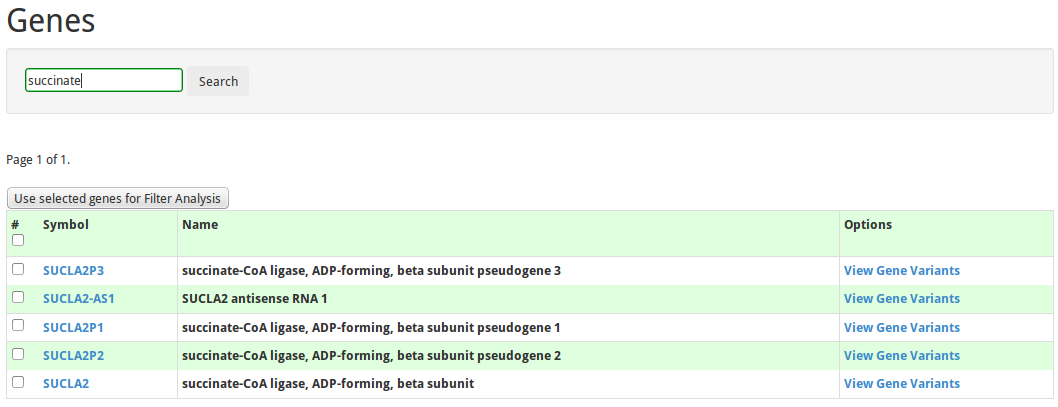
\includegraphics[width=1.5\textwidth]{./Figures/mendelmd/genes.png}}
  \caption[Interface para Busca de Genes]{Essa interface foi desenvolvida para permitir a busca de genes específicos, após a obtenção do resultado é possível investigar variantes apenas na lista de genes desejada.}
  \label{fig:genes_search}
  \end{figure}
\end{landscape}


  \clearpage
}

Também foi desenvolvida um opção para armazenar listas de genes personalizadas como por exemplo, com genes que já estivessem associados com doenças Mendelianas dominantes e recessivas. A figura \ref{fig:gene_lists} apresenta as listas de genes que foram inseridas no Mendel,MD.

\afterpage{
  \begin{landscape}
\begin{figure}[p]
  \centering
  \Large\textbf{Interface com grupos de genes adicionados}\par\medskip
  \fbox{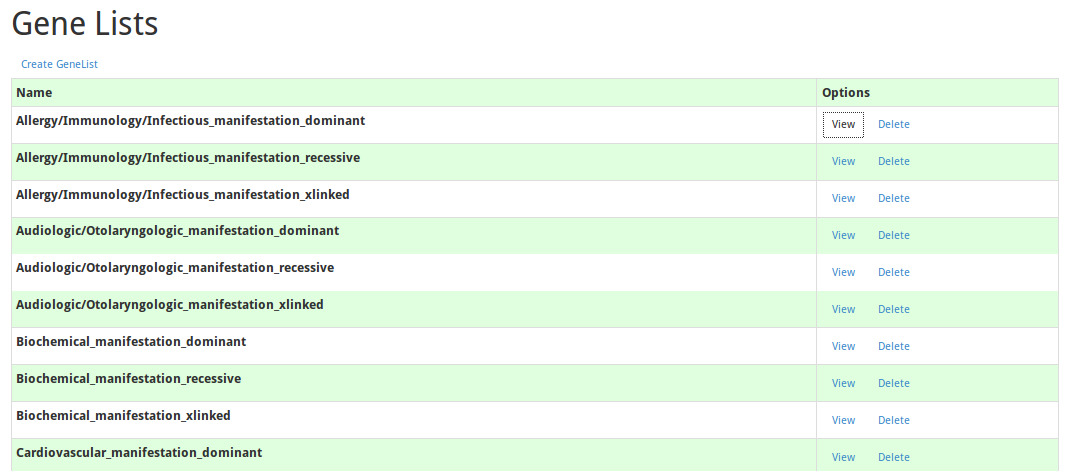
\includegraphics[width=1.5\textwidth]{./Figures/mendelmd/gene_lists.png}}
  \caption[Interface com grupos de genes adicionados]{Nesta interface podemos verificar os grupos de genes que foram criados pelos usuários de acordo com alguns critérios desejados.}
  \label{fig:gene_lists}
  \end{figure}
\end{landscape}

\clearpage
}

\subsection{Doenças}

Para obter dados sobre doenças Mendelianas nós utilizamos o site OMIM que possui atualmente 6845 doenças e 4715 genes. Esses dados foram inseridos no Mendel,MD para que fosse possível buscar por genes associados a doenças Mendelianas e para que eles pudessem ser inseridos no processo de filtragem de variantes.

Na figura \ref{fig:diseases} apresentamos a interface que permite a busca por doenças Mendelianas. Aqui é possível buscar por doenças e também selecionar os resultados para serem visualizados no método de filtragem de variantes na busca por variantes candidatas que estejam presentes nos indivíduos afetados pela doença. Nesta página o usuário pode digitar uma doença e selecionar todos os genes associados com ela para buscar variantes em seus indivíduos.

\afterpage{
  \begin{landscape}
\begin{figure}[p]
  \centering
  \Large\textbf{Interface para Busca de Doenças}\par\medskip
  \fbox{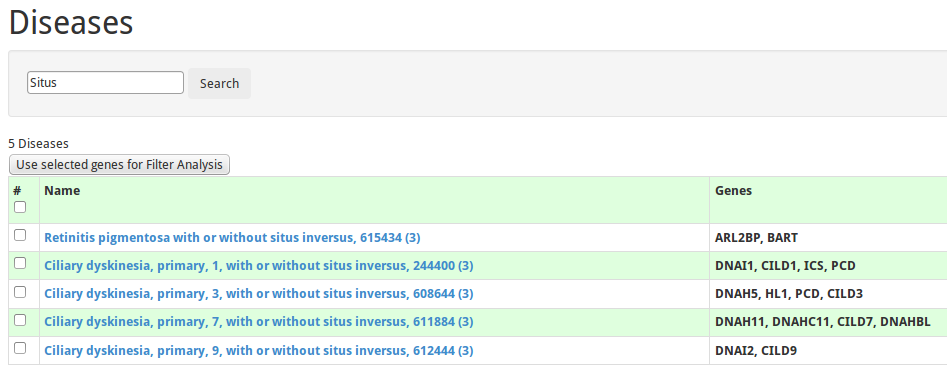
\includegraphics[width=1.5\textwidth]{./Figures/mendelmd/diseases.png}}
  \caption[Interface para Busca de Doenças]{Nesta interface podemos visualizar o resultado da busca por doenças com a palavra situs. A partir desta interface é possível visualizar variantes apenas em genes associados a um ou mais tipos específicos de uam determinada doença escolhida pelo usuário.}
  \label{fig:diseases}
  \end{figure}
\end{landscape}

\clearpage
}

\subsection{Filtragem de Variantes}

Após a anotação dos dados pelo sistema, o usuário pode filtrar as variantes dos indivíduos utilizando para essa tarefa um formulário web que permite a eliminação de variantes utilizando diferentes critérios de filtragem para tentar identificar a variante que possa ser responsável por causar a doença do paciente.

Este método foi implementado para permitir que essa tarefa pudesse ser repetida muitas vezes, facilitando a compreensão do que acontece durante cada etapa do processo e permitindo a combinação de diferentes opções de filtragem para chegar a uma lista pequena de candidatos.

As figuras a seguir ilustram o processo de filtragem implementado no Mendel,MD e que foram divididos em 3 etapas.
% 
% Step1Individuals.png
% Step2Variants.png
% Step3Databases.png
\afterpage{
  \begin{landscape}
\begin{figure}[p]
  \centering
    \Large\textbf{Filtragem de Variantes - 1ª Etapa}\par\medskip
    \fbox{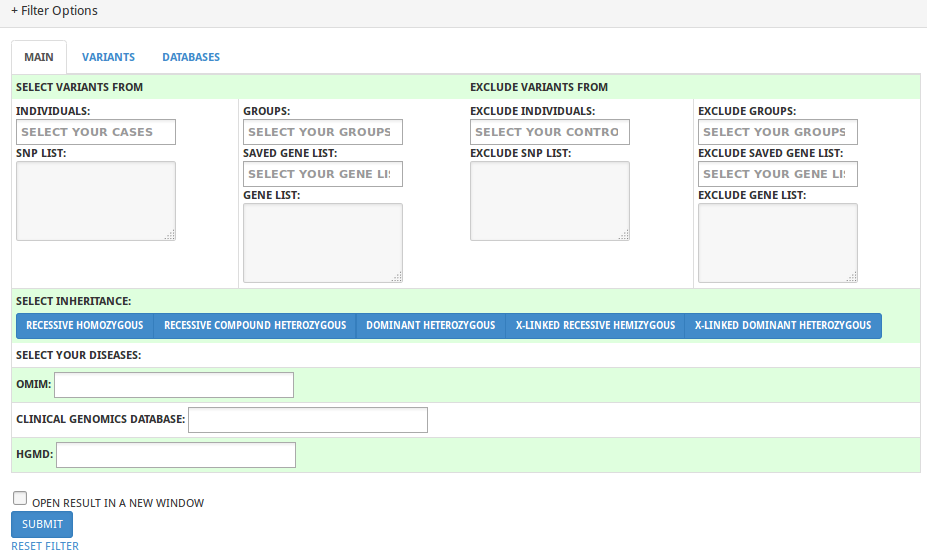
\includegraphics[width=1.3\textwidth]{./Figures/Filtragem/Step1Individuals.png}}
  \caption[Filtragem de Variantes - 1ª Etapa]{Essa é a primeira tela da filtragem de variantes onde o usuário precisa selecionar as opções referentes aos indivíduos, genes e snps que deseja analisar.}
  \label{fig:filtering_step1}
  \end{figure}
\end{landscape}

\clearpage
}

A figura \ref{fig:filtering_step1} mostra a primeira etapa onde o usuário pode selecionar os indivíduos em que gostaria de visualizar as variantes existentes e também os indivíduos que gostaria que fossem utilizados como controles no processo de exclusão de variantes. Além disso o usuário pode utilizar uma lista de genes e SNPs que gostaria de incluir ou excluir nos indivíduos selecionados.

\afterpage{
  \begin{landscape}
\begin{figure}[p]
  \centering
    \Large\textbf{Filtragem de Variantes - 2ª Etapa}\par\medskip
    \fbox{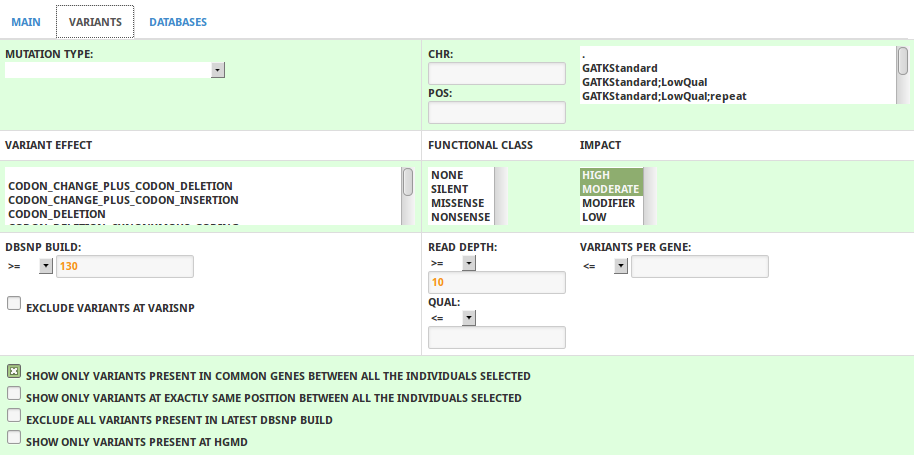
\includegraphics[width=1.5\textwidth]{./Figures/Filtragem/Step2Variants.png}}
  \caption[Filtragem de Variantes - 2ª Etapa]{Nesta interface é possível selecionar algumas opções das variantes presentes nos arquivos VCF.}
  \label{fig:filtering_step2}
  \end{figure}
\end{landscape}

\clearpage
}


Na figura \ref{fig:filtering_step2} apresentamos a segunda etapa onde o usuário possui diversas opções para definir sobre o tipo de variante que gostaria de visualizar nos resultados. A primeira opção seria em relação ao tipo de variante homozigótica (Ex. 1/1, 2/2 e 3/3) ou heterozigótica (Ex. 0/1, 0/2 e 0/3), esses números correspondem ao genótipos que foram codificados no arquivo VCF para cada indivíduo. Existe uma opção que foi desenvolvida para selecionar apenas variantes em um único cromossomo ou então em uma região específica de um cromossomo como por exemplo: chr:17, pos:80789468-80789469. Isso pode ajudar na investigação de regiões homozigóticas onde possam existir variantes candidatas.

Nesta aba o usuário também pode selecionar o tipo da mutação, o cromossomo, a posição, a coluna de filtro do VCF (Ex. PASS, LowQual), o efeito da variante, a classe funcional, o impacto, o dbSNP Build de quando a variante foi inserida no dbSNP, a cobertura, a qualidade, o número de variantes por gene, exibir apenas variantes presentes em genes comuns entre os indivíduos selecionados, mostrar apenas variantes que não estejam presentes no dbSNP, mostrar apenas variantes anotadas como \textit{``clinically associated''} pelo clinvar e também excluir variantes presentes em regiões com segmento de duplicação


\afterpage{
  \begin{landscape}
\begin{figure}[p]
  \centering
    \Large\textbf{Filtragem de Variantes - 3ª Etapa}\par\medskip
    \fbox{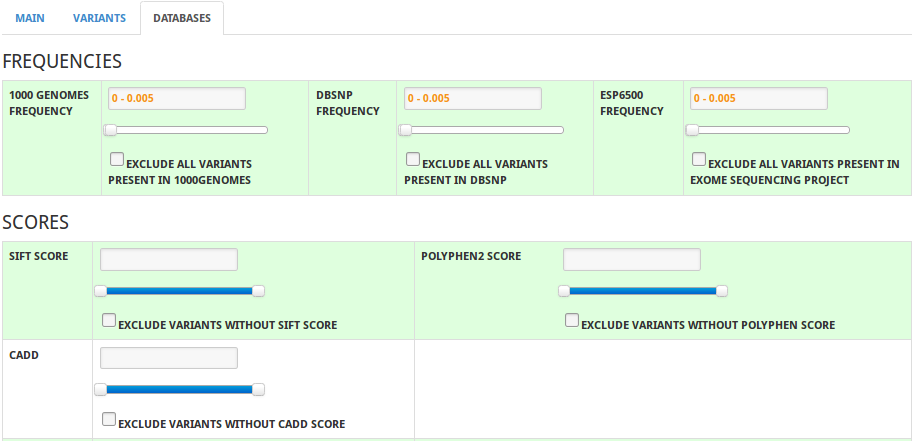
\includegraphics[width=1.5\textwidth]{./Figures/Filtragem/Step3Databases.png}}
  \caption[Filtragem de Variantes - 3ª Etapa]{Nesta interface é possível selecionar valores em relação aos Bancos de Dados e Escores de Priorização que foram anotados para cada variante.}
  \label{fig:filtering_step3}
  \end{figure}
\end{landscape}

\clearpage
}

Conforme apresentado na figura \ref{fig:filtering_step3}, a terceira etapa permite a filtragem utilizando valores de máximo e mínimo da frequência possível das variantes em bancos de dados como 1000Genomes, dbSNP e ESP6500. Por último foram incluídos filtros para se eliminar variantes utilizando os escores de SIFT e Polyphen-2.

Além disso, também é possível utilizar outras opções como por exemplo, apenas genes relacionados a doenças específicas do OMIM. Ao começar a digitar, usamos uma função \textit{autocomplete} que foi desenvolvida usando uma biblioteca de Javascript chamada de Select2 que retorna uma lista de doenças para que o usuário possa adicionar em suas pesquisa. Isso facilita muito a investigação de doenças que possuam um fenótipo parecido mas que sejam causadas por genes diferentes. Rapidamente podemos adicionar diversos nomes de doenças na pesquisa que o sistema irá encontrar apenas os genes relacionados a estas doenças. 

\subsubsection{1-Click}

Nesta interface foi desenvolvida uma configuração padrão de filtros que são recomendados para o início do processo de filtragem de variantes. Esta interface foi desenvolvida para facilitar e automatizar a identificação de variantes causadoras de doenças Mendelianas.

O método 1-Click foi inspirado em uma opção da ferramenta de análise filogenética Phylogeny.fr e permite que o usuário selecione apenas os indivíduos da análise e o tipo de herança genética mais provável o que reduz drasticamente o número de variantes candidatas para tentar encontrar a real causadora da doença do indivíduo. Este método faz com que os filtros sejam configurados automaticamente para o usuário. Esses valores foram definidos de maneira empírica e são apenas uma sugestão sobre como realizar a configuração dos filtros.

As configurações pré-definidas estão listadas a seguir:

\begin{itemize}
  \item SnpEff Impact: HIGH ou MODERATE
  \item Profundidade de Leitura maior ou igual a 10
  \item Mostrar apenas variantes em genes comuns aos indivíduos selecionados
  \item Excluir Variantes presentes no banco VariSNP
  \item Frequência da variante no 1000Genomes menor que 0.005
  \item Frequência da variante no dbSNP137 menor que 0.005
  \item Frequência da variante no Exome Variant Server menor que 0.005
\end{itemize}

\subsubsection{Análise de Filtros para Famílias}

Este método permite a análise de famílias (Ex. Trios, Quartetos e etc) que podem ser utilizadas no processo de filtragem para encontrar variantes que sejam heterozigóticas nos pais dos indivíduos e que sejam homozigóticas nos filhos afetados. Isso também permite a identificação de variantes candidatas que tenham um padrão de herança chamado de heterozigoto composto, ou seja, quando o filho recebe um alelo do gene com defeito de cada um dos pais. Além disso esta opção também permite a visualização de variantes chamadas \textit{de novo}, ou seja, aquelas que estão presentes nos filhos mas que obrigatoriamente não estejam presentes em nenhum dos pais selecionados.

Para isso nós desenvolvemos uma interface onde é possível definir quem são os pais dos pacientes durante a análise. Então este método usa essa informação obtida para eliminar as variantes que estejam presentes nos pais e que não obedeçam aos critérios de herança estabelecidos. Na figura \ref{fig:family_analysis} podemos observar o formulário para este tipo de análise, e na figura \ref{fig:family_analysis_results} podemos verificar que nos resultados para cada genótipo encontrado nos filhos existe o genótipo de cada um dos pais. Quando selecionamos por exemplo a opção 'heterozigoto composto' o que acontece por trás é que o sistema mostra nos resultados apenas genes candidatos que possuem pelo menos uma variante de cada um dos pais. Esse tipo de análise ajuda muito a reduzir o número de genes candidatos.


\afterpage{
\begin{landscape}
\begin{figure}[p]
  \centering
    \Large\textbf{Interface do Family Analysis}\par\medskip
  \fbox{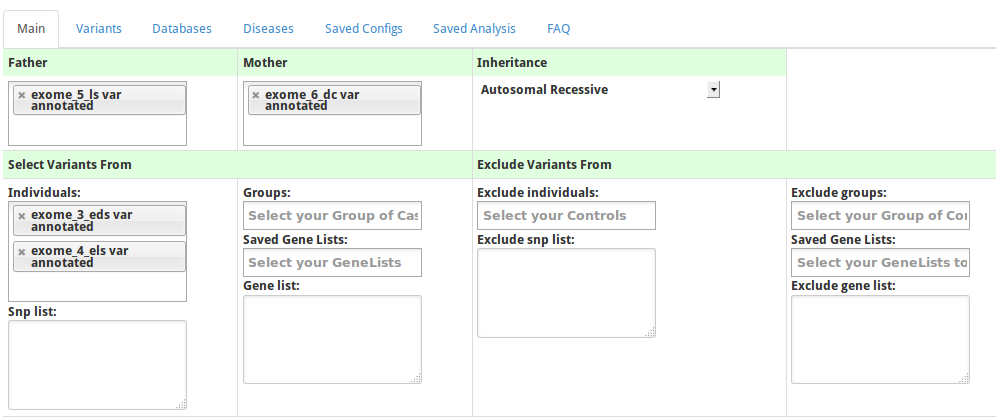
\includegraphics[width=1.5\textwidth]{./Figures/mendelmd/family_analysis.png}}
  \caption[Family Analysis]{Family Analysis - Neste formulário é possível selecionar quem são os pais dos indivíduos que estão sendo analisados para usar essa informação na hora da filtragem de dados}
  \label{fig:family_analysis}
\end{figure}
\clearpage
\end{landscape}
}




\afterpage{
\begin{landscape}
\begin{figure}[p]
  \centering
    \Large\textbf{Resultado do Family Analysis}\par\medskip
    \fbox{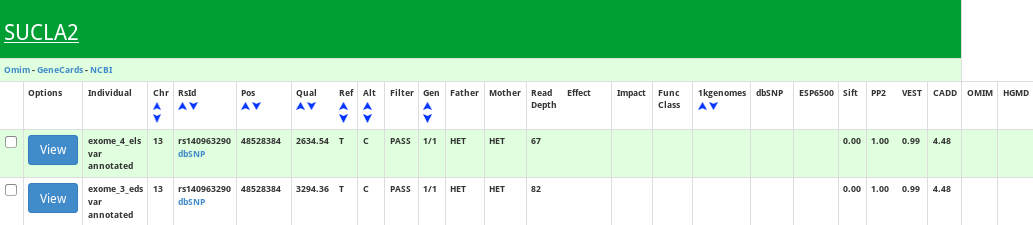
\includegraphics[width=1.5\textwidth]{./Figures/mendelmd/family_analysis_results.png}}
  \caption[Resultado do Family Analysis]{Nos resultados do Family Analysis é possível visualizar o genótipo de cada um dos pais para cada indivíduo nos resultados da análise}
  \label{fig:family_analysis_results}
\end{figure}
\end{landscape}

\clearpage
}
% 
% \subsubsection{Filter Pathway Analysis}
% 
% Este método mostra as variantes do resultado agrupadas por vias metabólicas do Kegg.  Isso permite a busca por variantes que estejam possivelmente associadas com uma única via metabólica. Para validar esta técnica utilizamos duas doenças chamadas Síndrome de \textit{Hurler} e de \textit{Hunter} que são causadas por mutações em genes diferentes (IDUA e IDS) mas que ambos os genes pertencem a via metabólica de glicosaminoglicanos. Na figura \ref{fig:pathway_analysis} podemos verificar que os resultados da análise estão agrupados por vias metabólicas. 
% 
% \afterpage{
% \begin{figure}[p]
%   \centering
%   \caption[Pathway Analysis]{Pathway Analysis - O resultado da filtragem aparece agrupado por vias metabólicas do KEGG}
%     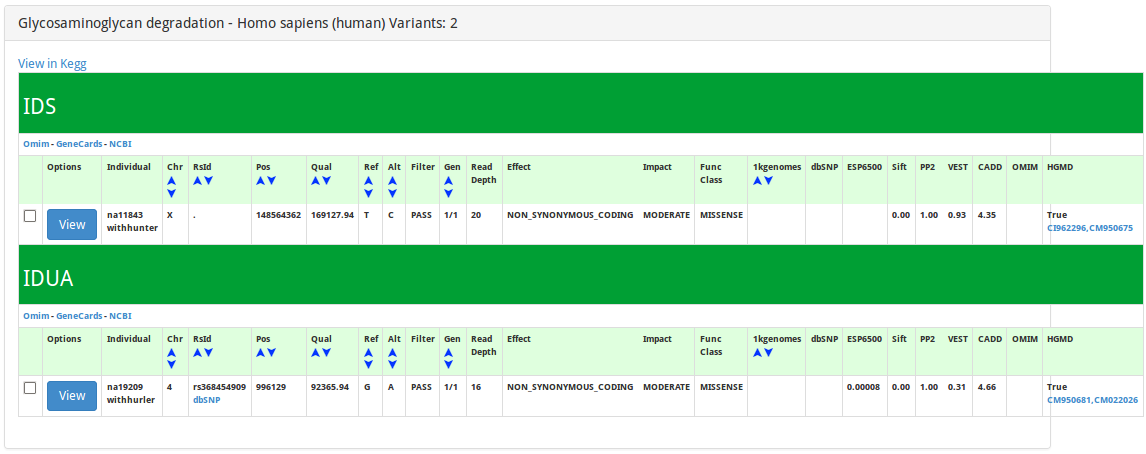
\includegraphics[width=1.0\textwidth]{./Figures/mendelmd/pathway_analysis.png}
%   \label{fig:pathway_analysis}
% \end{figure}
% \clearpage
% }

\subsubsection{Visualização de variantes}

Ao encontrar uma variante de interesse é possível verificar todas as informações disponíveis sobre aquela variante no sistema clicando no botão ''View``. Para isso nós desenvolvemos uma interface que mostra todos os campos do banco de dados para aquela variante específica. Esta interface possui centenas de anotações para cada variante.

\subsubsection{Exportação de resultados}

Após o usuário realizar a filtragem dos dados do paciente é possível exportar as variantes restantes em formato csv clicando sobre o botão ''\textit{export to csv}`` para que elas possam ser investigadas manualmente por um clínico utilizando programas como por exemplo o Excel.

\subsection{Comparação de Exomas}

Para possibilitar a comparação de exomas de diferentes indivíduos e até mesmo de exomas do mesmo indivíduo gerados a partir de tecnologias diferentes foi desenvolvido um método de comparação de VCFs. O algoritmo implementado nesta comparação possui duas etapas: primeiro procura apenas por posições que sejam comuns aos dois indivíduos sendo comparados, depois verifica se o genótipo nessas posições é igual ou diferentes entre os dois arquivos.

Na figura \ref{fig:comparison} podemos observar a comparação do genótipo de dois irmãos (Exome\_2\_MB e Exome\_3\_EDS) através deste método. Nesta caso nós encontramos 48.110 variantes em posições em comum entre os dois irmãos sendo que 84.2\% dessas variantes tinham o mesmo genótipo nos dois indivíduos selecionados.

\afterpage{
\begin{landscape}
\begin{figure}[p]
  \centering
    \Large\textbf{Interface para comparação de indivíduos}\par\medskip
  \fbox{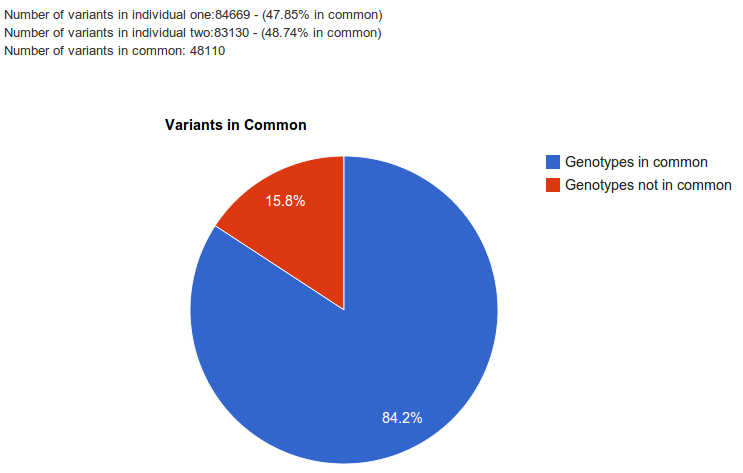
\includegraphics[width=1.3\textwidth]{./Figures/mendelmd/comparison.png}}
  \caption[Interface para comparação de indivíduos]{Essa interface foi desenvolvida para permitir a comparação de dois indivíduos ou VCFs.}
  \label{fig:comparison}
\end{figure}
\end{landscape}

\clearpage
}

%aqui termina construção mendel,md

\section{Casos Clínicos}

Nesta seção iremos discutir dois casos casos clínicos que foram recebidos para estudo pelo Laboratório de Genômica Clínica da Faculdade de Medicina da UFMG.

\subsection{Caso Clínico LGC 1}

O paciente RMS foi diagnosticado com duas doenças raras e pouco conhecidas \textit{situs inversus totalis} e panhipopituitarismo. 

\textit{Situs Inversus Totalis} é uma doença congênita onde todos os órgãos internos do indivíduo encontram-se invertidos, como exemplo, o coração encontra-se localizado no lado direito do peito ao invés do lado esquerdo. Este doença geralmente é acompanhada de problemas no trato respiratório, infertilidade, infecções no aparelho auditivo, e redução ou ausência de olfato. Estes problemas são causados por defeitos nos cílios e flagelos das células, sendo que um cílio é composto por um grupo de microtúbulos que são organizados em pares chamados de braços de dineína, recobertos por uma membrana chamada axonema. A ausência ou anormalidade dos braços de dineína conectando os nove pares de microtúbulos pode ser revelada através de uma microscopia eletrônica da célula. Apesar desta ser geralmente uma doença autossômica recessiva, ela também pode ser causada por mutações no cromossomo X \cite{Gebbia1997}.

Esta doença foi desenhada pela primeira vez por Leonardo da Vinci entre os períodos de 1452–1519, e foi reconhecida por Marco Aurélio Severino em 1643, porém, só foi descrita de uma maneira mais científica em 1793 por Matthew Baillie em seu livro "The Morbid Anatomy of Some of the Most Important Parts of the Human Body". Acredita-se que a incidência desta doença seja de 1 em cada 10.000 nascimentos. \cite{Report,Halasz2008}

Atualmente existem diversos genes associados com esta doença como por exemplo \textit{DNAI1, DNAH5, DNAH11, ZIC3 e CCDC11, IVS} \cite{Neesen2001,Olbrich2002, Bartoloni2002, Gebbia1997, Perles2012}.

Panhipopituitarismo é uma doença caracterizada pela ausência total ou parcial da glândula pituitária, o que provoca uma deficiência na produção de todos hormônios relacionados a este órgão. Este doença pode ser causada tanto por defeitos genéticos congênitos (presentes desde o nascimento) quanto por acidentes que danifiquem o hipotálamo ou a hipófise do indivíduo.

Entre os genes associados a esta doença podemos citar: \textit{HESX1, SOX2, SOX3, GLI2, LHX3, LHX4, PROP1, POU1F1} \cite{Viaroli2012}.

Um caso de panhipopituitarismo com situs inversus totalis foi descrito pela literatura em um paciente Húngaro de 56 anos\cite{Halasz2008}. Neste artigo o autor realizou o sequenciamento dos genes \textit{PIT1, PROP1, PITX2} a procura de mutações que pudessem estar relacionadas com a doença e no final eles concluíram não ter encontrado nenhuma mutação que pudesse ser responsável pelas doenças. Após a publicação deste artigo foi realizado o sequenciamento do exoma deste paciente e os dados foram compartilhados com nosso laboratório para análise junto com o exoma do nosso paciente RMS. A análise em conjunto desses dados não levou a nenhuma conclusão sobre uma mutação, ou gene, que pudesse ser compartilhado pelos dois indivíduos.

Além deste caso descrito pela literatura, outra paciente feminina de Boston, também foi diagnosticada com situs inversus totalis e panhipopituitarismo. Nós também recebemos os exomas dela e de sua família (pai, mãe e irmão) totalizando um quarteto de exomas que também foram analisados por nossa ferramenta a procura de mutações que pudessem ser compartilhadas entre os indivíduos afetados.

O tempo total de execução do pipeline completo para o indivíduo RMS foi de 12 horas.

Na tabela~\ref{rms_filtering_process} apresentamos o processo de filtragem de variantes sob um modelo recessivo que utilizado para o indivíduo RMS.

\afterpage{
\begin{table}[p]
\caption{Processo de Filtragem utilizado para o paciente RMS}
\begin{center}
\begin{tabular}{|p{9cm}|p{2.5cm}|p{2.5cm}|}
\hline
\textbf{Método de filtragem utilizado} & \textbf{Número de Variantes} & \textbf{Número de Genes} \\ \hline
Valores iniciais & 39.677 & 12.341 \\ \hline
Apenas variantes com o filtro PASS no VCF dos individuos. & 36.362 & 11.840 \\ \hline
Remoção de variantes encontradas em 292 exomas usados como controle. & 11.737 & 5.112 \\ \hline
Apenas variantes homozigóticas diferentes da referência Ex. 1/1, 2/1, 1/2. & 3.916 & 2.266 \\ \hline
Apenas variantes não sinônimas & 753 & 487 \\ \hline
Apenas variantes com um profundidade de leitura maior do que 10 (para uma cobertura média de 30X). & 644 & 428 \\ \hline
Apenas variantes em genes que possuem <=2 variantes por gene. & 434 & 386 \\ \hline
Remoção de variantes em regiões de segmento de duplicação. & 368 & 328 \\ \hline
Apenas variantes com frequência  menor do que 0.5\% nos indivíduos do 1000Genomes & 14 & 13 \\ \hline
Apenas variantes com frequência menor do que 0.5\% no dbSNP137 & 14 & 13 \\ \hline
Apenas variantes com frequência menor do que 0.5\% nos indivíduos do projeto ESP6500 & 8 & 8 \\ \hline
Apenas variantes com escore de SIFT entre 0  e 0.05 (Damaging) & 2 & 2 \\ \hline
Apenas variantes com escore de Polyphen-2 entre 0.85 e 1.0 (Damaging) & 1 & 1 \\ \hline
\end{tabular}
\end{center}
\label{rms_filtering_process}
\end{table}
\clearpage
}

Ao final da análise o gene restante \textit{GLRA4}, é um receptor de glicina alpha 4 e que não encontra-se associado a nenhuma das duas síndromes em estudo. Portanto, neste caso o mais recomendado seria aumentar o número de genes candidatos. A partir do momento que o número de genes obtidos estiver suficientemente pequeno, o usuário já pode investigar os genes um a um, para verificar se algum deles pode estar associado com a doença em estudo. 

Podemos observar que nenhum dos 13 genes candidatos (\textit{ZNF674}, \textit{C21orf62}, \textit{GPRIN2}, \textit{U52112.12}, \textit{OR52I1}, \textit{GLRA4}, \textit{VIL1}, \textit{DSPP}, \textit{HEPH}, \textit{TMEM199}, \textit{RP1L1}, \textit{SARM1}, \textit{PRR21}) pareceu estar associado com a doença, que nenhum deles foi descrito anteriormente como sendo o causador de nenhuma das duas doenças que foram diagnosticadas no indivíduo.

Apesar de todos os esforços não foi possível encontrar as causas destas doenças no paciente. Até mesmo a hipótese de que as variantes responsáveis possam estar em genes diferentes foi levantada devido a grande variedade de genes que poderiam ser responsáveis por causar ambas as doenças como por exemplo os genes \textit{OR52I1, GLRA4, VIL1 e DSPP}.

Este caso clínico foi importante para aprendermos a trabalhar com os dados de exomas e para automatizarmos o processo de análise para os futuros casos clínicos que seriam recebidos pelo nosso laboratório.

\subsection{Caso Clínico LGC 2}

Este caso clínico foi composto por 4 indivíduos de uma mesmo família, sendo dois irmãos (Exome\_3\_EDS e Exome\_4\_ELS) que haviam sido diagnosticados com síndrome de Leigh (OMIM:256000) e os seus pais (Exome\_5\_LS e Exome\_6\_DC) que não eram afetados pela doença.

A síndrome de Leigh possui 16 genes conhecidos no OMIM que podem conter variantes responsáveis por causar a doença, portanto este foi um caso ideal onde o sequenciamento e análise de exomas facilitou bastante o diagnóstico do paciente. 

A figura ~\ref{fig:sucla2} mostra os passos que foram utilizados para identificação da variante candidata no gene \textit{SUCLA2}.

Na figura \ref{fig:sucla2_view} nós apresentamos a visualização das variantes desta família em todos os cromossomos do genoma humano.

\afterpage{
\begin{figure}[p]
  \centering
    \Large\textbf{Processo de filtragem de variantes do caso LGC 2}\par\medskip
    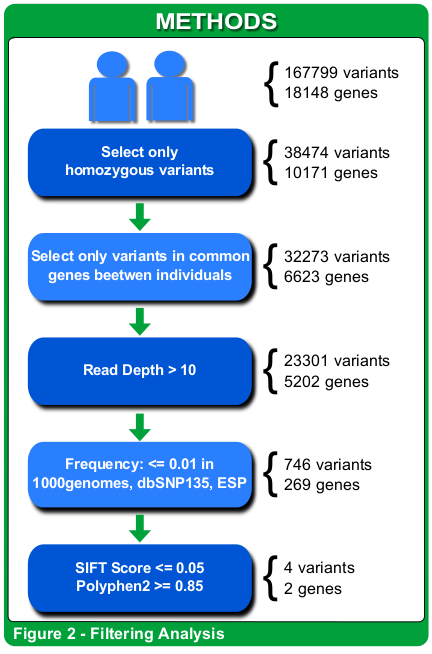
\includegraphics[width=0.8\textwidth]{./Figures/SUCLA2_filtering_process.png}
  \caption[Processo de filtragem de variantes do caso LGC 2]{Nesta figura podemos observar o que aconteceu com o número de variantes e genes em cada etapa da filtragem para este caso clínico.}
  \label{fig:sucla2}
\end{figure}
\clearpage
}


\afterpage{
\begin{landscape}

\begin{figure}[p]
  \centering
    \Large\textbf{Visualização das variantes do caso LGC 2}\par\medskip
    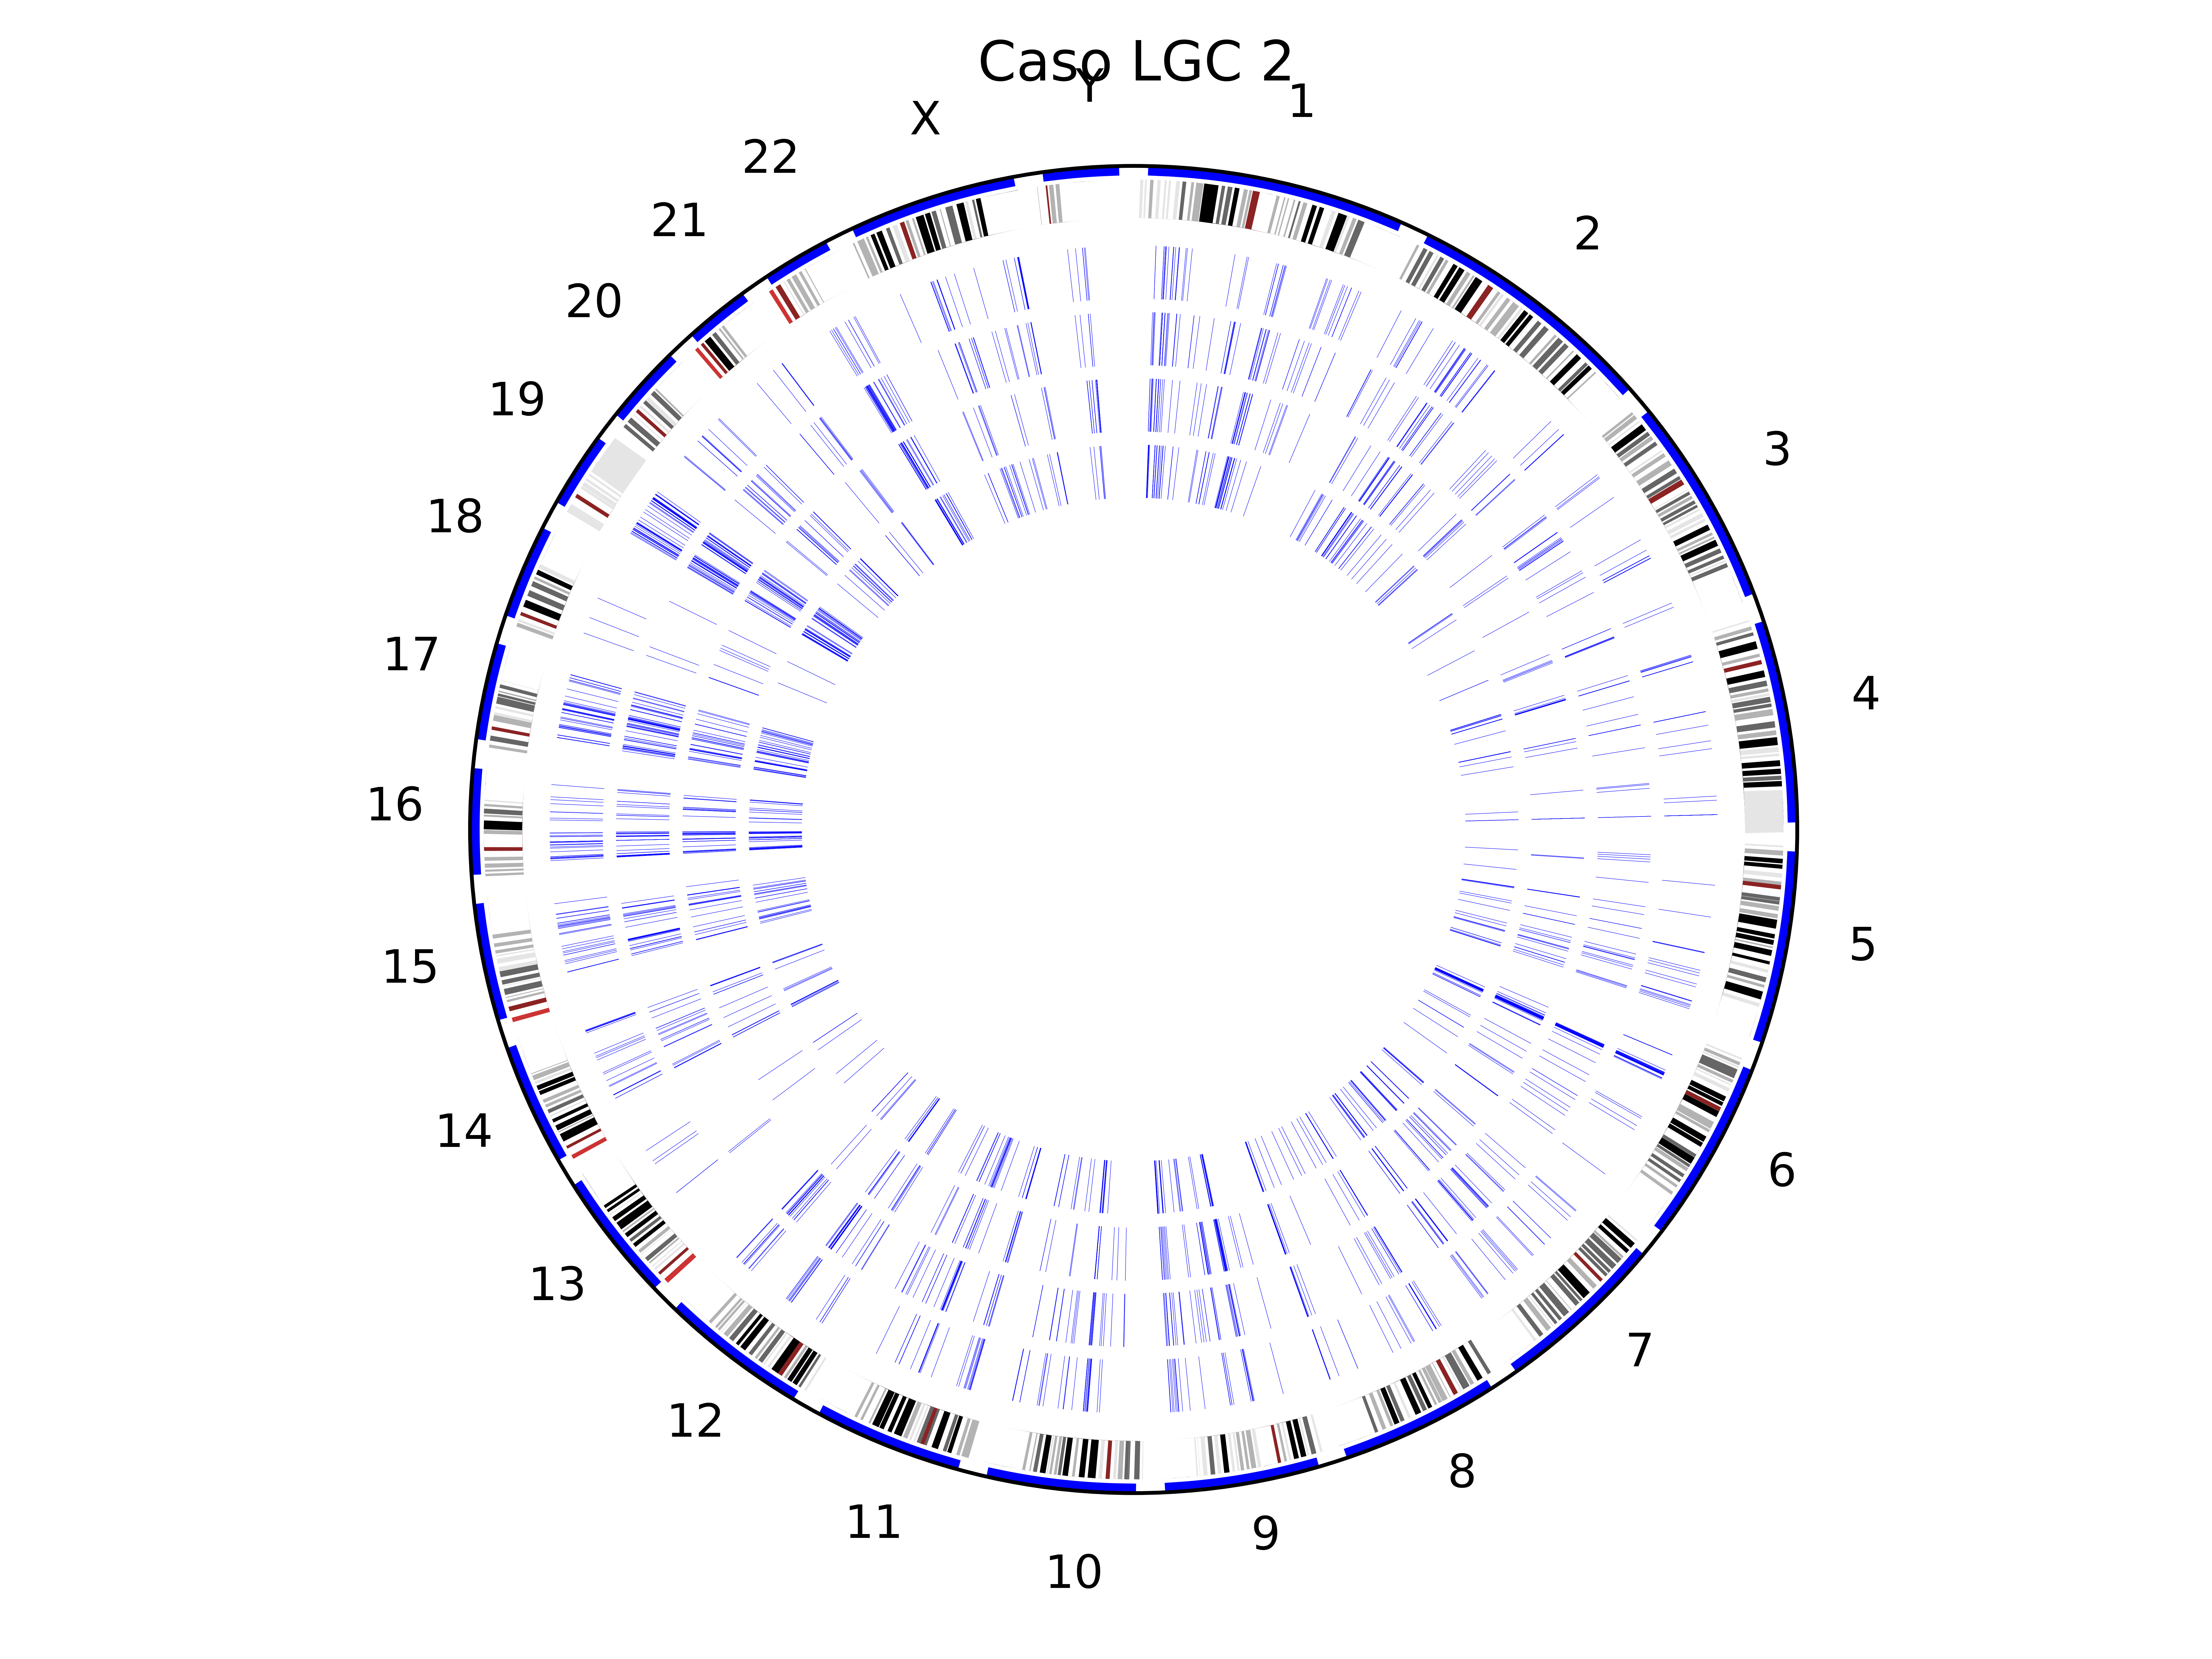
\includegraphics[width=1.0\textwidth]{./Figures/case_lgc_2.png}
  \caption[Visualização das variantes do caso LGC 2]{Esta figura foi criada como uma representação as variantes para o caso LGC 2 - Os indivíduos Exome\_3\_EDS, Exome\_4\_ELS, Exome\_5\_LS e Exome\_6\_DC estão representados no sentido de dentro para fora da imagem.}
  \label{fig:sucla2_view}
\end{figure}
\end{landscape}
\clearpage
}


Nesta análise foram identificados 2 genes candidatos: \textit{SUCLA2} e \textit{OR5H2}. Uma pesquisa bibliográfica revelou um artigo publicado em 2007 \cite{Carrozzo2007} com mutações no gene \textit{SUCLA2} associadas com \textit{Leigh-Like Syndrome}(OMIM:612073).

Esse foi o primeiro caso clínico em que conseguimos identificar uma nova mutação, em um gene \textit{SUCLA2} (GENEID:8803) que já havia sido descrito pela literatura como associado a uma doença Mendeliana. Esse caso mostrou que mesmo que fossem sequenciados todos os genes conhecidos associados a síndrome de Leigh, ainda assim a verdadeira mutação causadora da doença do paciente não seria encontrada.

Este caso também mostrou que o principal objetivo da filtragem de variantes não seria a identificação de um único gene candidato no final do processo mas o ideal seria retornar uma lista de genes e variantes que pudessem ser analisadas separadamente pelo médico ou pesquisador, que então seria capaz de identificar o gene e mutação responsável pela doença a partir de uma lista de possíveis candidatos.

A mutação encontrada no gene \textit{SUCLA2} foi confirmada por PCR e estudos funcionais mostraram que ela seria a real causadora da doença do paciente.

\subsection{Outros casos clínicos}


No dia 17 de maio de 2012 foram recebidos 12 novos exomas de 5 casos clínicos diferentes. A identificação dos exomas recebidos e uma breve descrição de seus casos clínicos são apresentados na tabela a seguir.

\afterpage{
\begin{landscape}

\begin{table}[p]
\caption{Descrição dos 12 exomas recebidos} % title of Table
\centering % used for centering table
\scalebox{1.2}{

    \begin{tabular}{|p{3cm}|p{11cm}|}
    \hline
    \textbf{Identificação}               & \textbf{Descrição}                                                                                   \\ \hline
    Exome\_1\_HJ                         & Paciente com uma calcificação no cérebro                                                    \\ \hline
    Exome\_2\_MB                         & Paciente (não relacionado com Exome\_1\_HJ) também com uma calcificação no cérebro \\ \hline
    Exome\_3\_EDS                        & Paciente com diagnóstico de Síndrome de Leigh (caso 2)                                  \\ \hline
    Exome\_4\_ELS                        & Irmão do indivíduo Exome\_3\_EDS também afetado pela mesma doença (caso 2)                                               \\ \hline
    Exome\_5\_LS                         & Mãe normal dos indivíduos Exome\_3\_EDS e Exome\_4\_ELS (caso 2)                                               \\ \hline
    Exome\_6\_DC                         & Pai normal dos indivíduos Exome\_3\_EDS e Exome\_4\_ELS (caso 2)                                               \\ \hline
    Exome\_7\_EUF                        & Paciente com o diagnóstico de Esclerose Tuberosa                                            \\ \hline
    Exome\_8\_MF                         & Mãe do paciente Exome\_7\_EUF diagnosticada com Síndrome de Marfan \\ \hline
    Exome\_9\_ELF                        & Mãe normal da paciente Exome\_8\_MF                                                                  \\ \hline
    Exome\_10\_EF                        & Pai normal da paciente Exome\_8\_MF                                                                  \\ \hline
    Exome\_11\_AP                        & Pai normal do indivíduo RMS                                                                        \\ \hline
    Exome\_12\_IN                        & Mãe normal do indivíduo RMS                                                                        \\ \hline
    \end{tabular}
}    
\end{table}
\end{landscape}

\clearpage
}

Esses 12 exomas foram sequenciados utilizando o sequenciador SOLID modelo 5500xl e o kit para o enriquecimento das regiões exônicas que utilizado foi o ``SureSelect V3'' da Nimblegen. Cada um desses exomas possuem uma cobertura média de 35X e o número médio de variantes por exoma foi de 80 mil. Este número de variantes é considerado um pouco alto em relação ao número variantes de exomas sequenciados por outras tecnologias. Isso é um problema bastante conhecido dos sequenciadores da plataforma SOLID.

Além dos exomas dos casos descritos neste trabalho muitos outros foram recebidos pelo nosso laboratório e foram analisados por outros pesquisadores do nosso laboratório utilizando para isso o Mendel,MD. Em especial \cite{Linhares2014b} e \cite{Linhares2014} são exemplos de dois casos clínicos do nosso laboratório que foram publicados. O primeiro caso, foi de dois irmãos afetados por uma doença chamada de leiomiomatose que é caracterizada pela proliferação de tumores  do músculo liso para outras regiões do corpo como pélvis e abdômen. Foram encontradas variantes em dois genes \textit{NDRG4 e RLTPL}. No segundo caso tivemos dois irmãos com miofibromatose infantil onde foram encontradas variantes nos genes \textit{PDGFRB e PTPRG}, sendo que as variantes do gene \textit{PDGFRB} foram herdadas da mãe e as variantes do gene \textit{PTPRG} foram herdadas do pai. Foi sugerido que a mãe dos pacientes apesar de possuir a mesma mutação não seria afetada pela doença o que caracteriza um modelo de penetrância incompleta para este caso clínico.

Através do uso do Mendel,MD foi possível levantar muitas hipóteses sobre as possíveis variantes que poderiam estar associadas a síndromes que ainda não haviam sido descritas pela literatura. Em colaboração com o Laboratório GENE - Núcleo de Genética Médica, foram sequenciados e analisados 57 casos que ainda não possuíam um diagnóstico definitivo ou onde havia uma suspeita de que os paciente pudessem ter doenças mendelianas.

Em 29 dos 57 casos clínicos analisados (51\%) foi possível chegar a um diagnóstico definitivo após utilizar o Mendel,MD para analisar o exoma dos pacientes. 

Além dos nossos próprios casos, a pesquisadora Dra. Judith Conroy do Children'n University Hospital em Dublin utilizou o Mendel,MD para analisar casos de 42 crianças com encefalopatia epilética infantil precoce. Ela conseguiu encontrar variantes patogênicas em 26\% dos pacientes o que estaria próximo dos valores de sucesso desta metodologia de acordo com a literatura \cite{Yang2013b}.

\section{Mendel,MD - Validação}

Apesar do Mendel,MD ter auxiliado no diagnóstico de muitos casos clínicos do nosso próprio laboratório, ainda seria necessário realizar uma validação utilizando exomas de casos clínicos que já fossem descritos pela literatura, onde o gene e a mutação responsáveis por causar a doença já estivessem identificados e validados experimentalmente.

Para isso nós fizemos uma pesquisa no Pubmed procurando por artigos científicos que utilizaram o sequenciamento de exomas nos dois últimos anos para estudar doenças Mendelianas e com isso criamos uma lista de 100 artigos que foram selecionados. Depois da criação desta lista, nós enviamos e-mails para os autores dos estudos pedindo que os genótipos dos pacientes fossem compartilhados com o objetivo de fazer uma validação do Mendel,MD utilizando dados da literatura.

O objetivo principal desta validação foi verificar se os usuários do Mendel,MD seriam capazes de identificar o gene, a variante e a doença do paciente em cada caso clínico, utilizando os dados do exoma do paciente. 

Na tabela~\ref{Casos_validacao} apresentamos uma lista com os exomas recebidos e que foram utilizados neste processo de validação do Mendel,MD.
Ao todo nós recebemos 19 exomas de 11 casos clínicos diferentes. Esses dados foram padronizados para o formato VCF e foram inseridos no Mendel,MD através da nossa interface de upload.

A seguir nós descrevemos brevemente como cada caso clínico foi analisado. Em primeiro lugar nós definimos os valores mínimos de profundidade de leitura de acordo com a cobertura média obtida para cada um dos exomas.

\afterpage{
\begin{landscape}

\begin{table}[p]
\caption{Casos Recebidos para Validação}
\begin{center}
\scalebox{1.2}{
\begin{tabular}{|l|l|l|}
\hline
\textbf{Casos Clínicos} & \textbf{Indivíduos} & \textbf{Modelo de Herança da doença} \\ \hline
1 & DG00658 & Autossômica Recessiva \\ \hline
2 & P6NV & Autossômica Recessiva \\ \hline
3 & P2 & Autossômica Recessiva \\ \hline
4 & NI1000380 e NI1001037 & Autossômica Dominante \\ \hline
5 & 924 3037 e 3121 & Autossômica Dominante \\ \hline
6 & NI40816, NI54126, NI48062, NI43664 & Autossômica Dominante \\ \hline
7 & DG1365 & Autossômica Recessiva \\ \hline
8 & P5 & Autossômica Recessiva (Heterozigoto composto) \\ \hline
9 & P3 & Autossômica Recessiva (Heterozigoto composto) \\ \hline
10 & S0001 & Autossômica Dominante \\ \hline
11 & child, father, mother & Autossômica Recessiva \\ \hline
\end{tabular}
}
\end{center}
\label{Casos_validacao}
\end{table}
\end{landscape}

\clearpage
}  

Para realizar na validação dos casos primeiramente nós pedimos para um médico criar uma lista com os sintomas para cada caso clínico.

\subsection{Caso 1}

Para o caso 1 nós recebemos o indivíduo DG00658 com uma doença autossômica recessiva. Este indivíduo tinha inicialmente 86.445 variantes e 63.25X de cobertura. Nós utilizamos o método 1-Click e como resultado nós obtivemos uma lista com mutações em 29 genes candidatos. Desses 29 genes, apenas 10 genes estavam presentes no OMIM como já sendo associados com doenças Mendelianas. 

Nós comparamos essa lista de genes associados a doenças com a lista de sintomas do paciente e selecionamos o \textit{POC1A} associado com a doença ``Short Stature, Onychodysplasia, Facial Dysmorphism, and Hypotrichosis'' como sendo um bom candidato. Esse gene tem uma mutação de G>A na posição 3-52183866 (R81*) com rsID rs397514487 que foi classificada pelo SnpEff com efeito STOP\_GAINED, impacto HIGH e classe funcional NONSENSE. É importante notar que esta mutação não possui escores de patogenicidade como SIFT e Polyphen-2 porque ela não causa uma mudança no aminoácido mas ela possui um CADD escore de 7.57, o que é um valor extremamente alto.

\subsection{Caso 2}

No caso 2 nós recebemos o individuo P6NV que tinha uma doença autossômica recessiva. Após realizar o 1-Click foram obtidos 10 genes candidatos, sendo que 4 já estavam presentes no OMIM. Comparando a lista de genes do individuo com a lista de sintomas nos selecionados o gene \textit{MRPL44} como sendo o melhor candidato para este caso clínico. 
Este gene possui uma mutação homozigótica no cromossomo 2 posição 224824538 (L156R) que é uma variante não-sinônima, missense com um SIFT de 0 e um Polyphen-2 de 0.95.

\subsection{Caso 3}

Nos caso três o indivíduo P2 foi diagnosticado com uma doença autossômica recessiva, após realizarm o 1-Click, foram obtidos 22 genes candidatos, sendo que 9 já estavam presentes no OMIM. Após investigar essa lista de genes nós selecionamos o gene \textit{AARS} como sendo o melhor candidato de acordo com a lista de sintomas definidos para este caso clínico. Este gene possui uma mutação homozigótica na posição 6:44272249 (R592W) que é não-sinônima, missense, com um SIFT de 0 e um Polyphen-2 de 0.81.

\subsection{Caso 4}

Para o caso 4 nós tinhamos dois indivíduos (nl1001037 e nl1000380) desta vez utilizando um modelo de herança dominante no 1-Click, nós encontramos 63 genes candidatos, sendo que 11 genes já estavam presentes no OMIM e por fim selecionamos o gene \textit{WDR35} como sendo o melhor candidato para este caso. Este gene tinha 3 mutações heterozigotas, sendo que uma foi encontrada no indivíduo nl1001037 na posição 2:20133230 (A875T) que era não-sinônima, missense, com um SIFT de 0 e um Polyphen-2 de 1.0. O outro indivíduo nl1000380 tinha duas mutações candidatas uma na posição 2:20145548 (E626G) sendo não sinônima e a outra na posiçao 2:20189045 em uma região de splicing.

\subsection{Caso 5}

Para o caso 5 com os indivíduos 924, 3037 e 3121 com uma doença autossômica dominante, nós utilizamos o 1-Click e encontramos 25 genes presentes no OMIM, a partir desta lista nós selecionamos o gene \textit{MAX} que continha 3 mutações no cromossomo 14 nas posições 65569057, 65544630, 65544703 em cada um dos indivíduos. Essa mutações são consideradas START\_LOST, SPLICE\_SITE\_DONOR e STOP\_GAINED respectivamente.


\subsection{Caso 6}

Para o caso 6 nós tivemos quatro indivíduos nl54126, nl48062, nl43664 e nl40816. Nós utilizamos o modelo de herança dominante para filtragem de variantes que retornou uma lista com 19 genes candidatos, desta lista apenas 4 genes estavam presentes no OMIM e o gene \textit{SETPB1} foi selecionado como sendo o melhor candidato baseado na lista de sintomas do paciente por possuir uma mutação em cada um dos indivíduos nas seguintes posições 18:42531914 (G870D), 18:42531907 (D868N), 18:42531907 (D868N) e 18:42531917 (I871T) todas consideradas MODERATE e MISSENSE.

\subsection{Caso 7}

No caso 7 nós tivemos apenas um único indivíduo DG1365. Utilizando o modelo de herança recessivo nós encontramos 23 genes candidatos, sendo apenas 4 genes já presentes no OMIM. Como nenhum dos candidatos se mostrou bom o suficiente, nós reduzimos o valor mínimo de profundidade de leitura para este caso e com isso identificamos o gene \textit{DOCK6} que parecia estar relacionado com a lista de sintomas deste caso clínico. Neste gene foi encontrada uma mutação na posição 19:11353955 LT454 que foi classificada pelo SnpEff como HIGH e frameshift. Este caso foi muito importante para mostrar que os valores padrões de filtragem nem sempre serão a melhor escolha.

\subsection{Casos 8 e 9}

Para os casos 8 e 9, nós recebemos dois indivíduos P3 e P5 mas nenhuma informação sobre a lista de sintomas dos pacientes, nós apenas sabíamos o modelo de herança que era heterozigoto composto. Um problema inicial na conversão dos dados para VCF fez com que a variante deste caso fosse excluída do arquivo inserido no Mendel,MD. Após as devidas correções no arquivo convertido nós conseguimos identificar as variantes corretas para estes dois casos clínicos.

Para o caso 8 nós obtivemos 46 genes, sendo que apeas 4 estavam associados com doenças no OMIM. Após considerar a lista de sintomas do paciente, o gene \textit{TK2} foi selecionado como sendo um bom candidato para validação. Este gene tinha duas mutações, a primeira na posição 16:66551110 (R225W) que era não-sinônima, com um SIFT escore de 0, Polyphen-2 de 0.97 e um escore de CADD de 2.53, e a segunda na posição 16:66551095 (T230A) com um SIFT escore de 0.15, Polyphen-2 de 0.06 e com um CADD escore de 1.94. 

Para o caso 9 nós utilizando o modelo de herança heterozigoto composto nós encontramos 28 genes sendo apenas 3 já associados com doenças Mendelianas. Nós selecionamos o gene \textit{FARS2} com duas mutações nas posições 6:5545494 (I329T) com um SIFT escore de 0.00, Polyphen-2 escore de 1.0 e com um CADD escore de 5.20, a segunda mutação foi encontrada na posição 6:5613508 (D391V) com um escore de SIFT de 0, um Polyphen-2 de 1 e um cadd escore de 2.25.

\subsection{Caso 10}

Para o caso 10, nós recebemos o paciente S0001 com um doença autossômica dominante, após utilizarmos o 1-Click nós obtivemos uma lista com 261 genes, sendo 51 genes já presentes no OMIM. Após comparar a lista de sintomas para este caso nós selecionamos o gene \textit{GJC2} que possui uma mutação na posição 1:228345602 (S48L) que é não-sinônima, MISSENSE com um SIFT escore de 0.14, um Polyphen-2 escore of 0.95 e um CADD escore de 4.01.

\subsection{Caso 11}

Para o caso 11, recebemos um trio de exomas (\textit{father, mother, children}) onde o filho do casal tinha uma doença autossômica recessiva. Após utilizarmos o 1-Click nós obtivemos 8 genes, sendo que apenas um gene já estava presente no OMIM. Após reduzirmos a quantidade mínima de profundidade de leitura para 5, nós identificamos 31 genes sendo que 6 já estavam presentes no OMIM. Dessa lista nós selecionamos o gene \textit{KIF1A} como sendo o melhor candidato. Este gene tinha uma mutação na posição 2:241723190 com um SIFT de 0, um Polyphen-2 de 0.60 e um CADD escore de 3.56. Este caso também serve como um exemplo de que devemos sempre verificar a cobertura média dos exomas antes de definirmos cada uma das opções de filtragem de variantes. A criança neste caso tinha uma cobertura de 23.52X o que seria uma boa indicação para reduzir o valor mínimo de profundidade de leitura.


\section{Validação da usabilidade da ferramenta}

Para comprovar a usabilidade do sistema, o Professor Sérgio Pena realizou um teste com suas alunas do curso de Bases Moleculares ministrado no Intituto de Ciências Biológicas (ICB) no segundo semestre de 2014. O objetivo desse teste foi verificar se outras pessoas também seriam capazes de analisar os casos clínicos e identificar o gene, a variante e a doença Mendeliana para cada caso usando para isso o Mendel,MD.

Cada aluna do curso recebeu um caso clínico para analisar e todas foram capazes encontrar as mutações corretas para cada caso clínico utilizando o Mendel,MD. Após o término dessa disciplina, foi elaborado um questionário que foi enviado para cada aluna com três perguntas para avaliarem o Mendel,MD de acordo com alguns critérios. A seguir apresentamos as perguntas que foram enviadas as alunas.

\begin{itemize}
 \item 1) Que nota geral você dá à sua experiência com o software Mendel,MD?
 \begin{itemize}
  \item A - 0-20
  \item B - 30-40
  \item C - 40-60
  \item D - 70-80
  \item E - 90-100
  \end{itemize}
 \item 2) Em termos de facilidade de uso em comparação com softwares que vocês estão acostumadas a usar, como você avaliaria o Mendel,MD?
 \begin{itemize}
  \item A - Muito fácil
  \item B - Fácil
  \item C - Médio
  \item D - Difícil
  \item E - Muito difícil
  \end{itemize}
 \item 3) Quais são as suas sugestões para melhora do Mendel,MD em facilidade de uso e eficiência?
  
\end{itemize}

Ao todo três alunas do curso responderam ao questionário que foi enviado por e-mail pelo Professor Sérgio Pena e as respostas obtidas para cada pergunta estão descritas a seguir. 

Na pergunta número um, as três alunas classificaram o Mendel,MD com uma nota geral: E (90-100). Isso significa que o Mendel,MD obteve uma boa qualificação em relação a experiência que os usuários tiveram com o sistema em geral.

Em relação a pergunta número dois sobre a facilidade de utilização do software nós obtivemos as seguintes respostas: A (Muito Fácil), B (Fácil) e B (Fácil). Isso mostra que obtivemos também um boa qualificação em relação a facilidade de uso do Mendel,MD.

Todas as sugestões que foram enviadas pelas alunas na pergunta descritiva número três foram levadas em consideração e ajudaram a melhorar a facilidade de uso do sistema. Essa validação que foi realizada ajudou a fornecer ainda mais evidência de que o programa poderia ser realmente utilizado por outros pesquisadores para realizar a identificação de mutações candidatas para estudar diferentes casos clínicos.
